\newif\ifdraft\drafttrue  % set true to show comments
\newif\iflastminute\lastminutetrue  % for things to check at the end
\newif\iflater\laterfalse  % for things to think about after submission

\documentclass[acmsmall,review,anonymous]{acmart}
\settopmatter{printfolios=true,printccs=false,printacmref=false}
% % For double-blind review submission, w/ CCS and ACM Reference
% \documentclass[acmsmall,review,anonymous]{acmart}\settopmatter{printfolios=true}
% % For single-blind review submission, w/o CCS and ACM Reference (max
% submission space)
% \documentclass[acmsmall,review]{acmart}\settopmatter{printfolios=true,printccs=false,printacmref=false}
% % For single-blind review submission, w/ CCS and ACM Reference
% \documentclass[acmsmall,review]{acmart}\settopmatter{printfolios=true} % For
% final camera-ready submission, w/ required CCS and ACM Reference
% \documentclass[acmsmall]{acmart}\settopmatter{}


% % Journal information % Supplied to authors by publisher for camera-ready
% submission; % use defaults for review submission.
\acmJournal{PACMPL}
\acmVolume{1}
\acmNumber{ICFP} % CONF = POPL or ICFP or OOPSLA
\acmArticle{1}
\acmYear{2018}
\acmMonth{1}
\acmDOI{} % \acmDOI{10.1145/nnnnnnn.nnnnnnn}
\startPage{1}

% % Copyright information % Supplied to authors (based on authors' rights
% management selection; % see authors.acm.org) by publisher for camera-ready
% submission; % use 'none' for review submission.
\setcopyright{none}
\usepackage{algorithm, amsmath, amssymb, verbatim, enumerate, graphicx,
  centernot, tikz, array, mathtools, bussproofs, stmaryrd, enumitem,
  stackengine, subcaption}
\captionsetup{compatibility=false}
\usepackage{relsize}
\usepackage{listings}
\usepackage{proof}
\usepackage{xspace}
\usepackage[noend]{algpseudocode}
\usepackage[capitalize]{cleveref}

\lstset{ language=Caml, basicstyle=\linespread{0.8}\upshape\sffamily,
keywordstyle=\upshape\sffamily\color{dkblue}, keepspaces=true,
framexleftmargin=1ex, framexrightmargin=1ex, showstringspaces=true,
commentstyle=\itshape\rmfamily,
emph={synth,collapse,perm,squash,normalize,using,ins,del,lens,let,get,put,rquot,lquot},
emphstyle=\upshape\sffamily\color{dkblue}, 
columns=fullflexible,
escapechar=\#,
mathescape, 
xleftmargin=1.5em,
% BCP: I find this distracting:
% stringstyle=\sffamily\color{dkred},
}
\makeatletter
     \let\lst@oldvisiblespace\lst@visiblespace
     \def\lst@visiblespace{\,\lst@oldvisiblespace\,}
\makeatother

% %%%% Macros Colors
\definecolor{dkblue}{rgb}{0,0.1,0.7}
\definecolor{dkgreen}{rgb}{0,0.6,0}
\definecolor{dkred}{rgb}{0.6,0,0}
\definecolor{dkpurple}{rgb}{0.7,0,0.4}
\definecolor{olive}{rgb}{0.4, 0.4, 0.0}
\definecolor{teal}{rgb}{0.0,0.5,0.5}
\definecolor{orange}{rgb}{0.9,0.6,0.2}
\definecolor{lightyellow}{RGB}{255, 255, 179}
\definecolor{lightgreen}{RGB}{170, 255, 220}
\definecolor{teal}{RGB}{141,211,199}
\definecolor{darkbrown}{RGB}{121,37,0}

\newcommand{\FINISH}[3]{\ifdraft\textcolor{#1}{[#2: #3]}\fi}
\newcommand{\bcp}[1]{\FINISH{dkred}{B}{#1}}
\newcommand{\BCP}[1]{\FINISH{dkred}{B}{\bf #1}}
\newcommand{\afm}[1]{\FINISH{dkgreen}{A}{#1}}
\newcommand{\dpw}[1]{\FINISH{dkblue}{D}{#1}} % Toronto Maple Leafs Blue :-)
\newcommand{\saz}[1]{\FINISH{orange}{SZ}{#1}}
\newcommand{\SAZ}[1]{\FINISH{orange}{SZ}{#1}}
\newcommand{\ksf}[1]{\FINISH{teal}{K}{#1}}
\newcommand{\sam}[1]{\FINISH{dkpurple}{SM}{#1}}

% For Inference Rules
\newcommand{\Rule}[2]{\infer{#2}{#1}}
\newcommand{\RuleSide}[3]{\infer[#3]{#2}{#1}}
% \newcommand{\Axiom}[1]{\Rule{}{#1}}

\newcommand{\wf}[1]{\ensuremath{#1\;\mathsf{wf}}}

% FOR Regular Expression names
\newcommand{\re}[1]{\ensuremath{\mathtt{#1}}}
\newcommand{\codefont}[1]{\ensuremath{\mathsf{#1}}}
\newcommand{\kw}[1]{\textcolor{dkblue}{\ensuremath{\mathsf{#1}}}}
\newcommand{\collapse}[2]{\ensuremath{\kw{collapse} \; #1 \mapsto #2}}
\newcommand{\squash}[3]{\ensuremath{\kw{squash} \; #1 \rightarrow #2\; \kw{using} \; #3}}
\newcommand{\perm}[2]{\ensuremath{\kw{perm}(#1)\; \kw{with}\; #2}}
\newcommand{\normalize}[3]{\ensuremath{\kw{normalize}(#1, #2, #3)}}
\newcommand{\eqrel}[1]{\ensuremath{\equiv_{#1}}}
\newcommand{\sep}{\ensuremath{\ | \ }}
\newcommand{\canonize}{\ensuremath{\kw{canonize}}}
\newcommand{\bibtex}{\textsc{Bib}\TeX{}}
\newcommand{\get}{\ensuremath{\kw{get}}}
\newcommand{\semicolon}{\ensuremath{\; ; \;}}
\newcommand{\lput}{\ensuremath{\kw{put}}}
\newcommand{\create}{\ensuremath{\kw{create}}}
\newcommand{\const}{\ensuremath{\kw{const}}}
\newcommand{\swap}{\ensuremath{\kw{swap}}}
\newcommand{\id}{\ensuremath{\kw{id}}}
\newcommand{\lquot}{\ensuremath{\kw{lquot}}}
\newcommand{\rquot}{\ensuremath{\kw{rquot}}}
\newcommand{\lift}{\ensuremath{\kw{lift}}}
\newcommand{\bsep}{\ \ \sep{} \ \ }

\newcommand{\Name}{Optometrist\xspace}

\newcommand{\QRESize}{\textbf{QS}}
\newcommand{\canonizeAndSpecSize}{\textbf{BS}}
\newcommand{\LensAndSpecSize}{\textbf{NS}}

%\newcommand{\QOpt}{Optician_Q}
\newcommand{\QOpt}{QRE-enhanced Optician}
\newcommand{\OpticianRuntime}{\textbf{Optician}}
\newcommand{\QREOptician}{\textbf{Optician\textsubscript{Q}}}
\newcommand{\SystemOnOptician}{\textbf{QO}}
\newcommand{\SystemOnBenchmarks}{\textbf{QQ}}
\newcommand{\cd}[1]{\lstinline[backgroundcolor=\color{white}]$#1$}


% %%%%%%%%%%%%%%%%%%%%%%%%%%%%%%%%%%

\begin{document}
\title{Synthesizing Quotient Lenses}
\begin{abstract}
{\em Quotient lenses} are bidirectional transformations whose correctness
laws are ``loosened'' by specified equivalence relations, allowing
inessential details in concrete data formats to be suppressed. 
For example, a programmer could use a quotient lens to define 
a transformation that ignores the order of fields in XML data, so
that two XML files with the same fields but in different orders would be
considered the same, allowing a single, simple program to handle them both. 
%
Building on a recently published algorithm for synthesizing plain bijective
lenses from high-level specifications, we show how to synthesize bijective
quotient lenses in three steps. First, we introduce {\em quotient regular
  expressions} (QREs), annotated regular expressions that conveniently mark
inessential aspects of string data formats; each QRE specifies,
simulteneously, a regular language and an equivalence relation on it.
Second, we introduce {\em QRE lenses}, i.e., lenses mapping between QREs.
Our key technical result is a proof that every QRE lens can be transformed
into a functionally equivalent lens that canonizes source and target data just
at the ``edges'' and that uses a bijective lens to map between the respective
canonical elements; no internal canonization occurs in a lens in this normal
form. Third, we leverage this normalization theorem to {\em synthesize} QRE
lenses from a pair of QREs and example input-output pairs, reusing earlier work
on synthesizing plain bijective lenses. We have implemented QREs and QRE lens
synthesis as an extension to the bidirectional programming language Boomerang.
We evaluate the effectiveness of our approach by synthesizing QRE lenses
between various real-world data formats in the Optician benchmark suite.
\end{abstract}

\keywords{quotient regular expressions, QRE lens, synthesis}
\maketitle

\section{Introduction}
Programmers often need to write programs that bidirectionally convert data
between two different formats. For example, bibliographic data may be stored in
\bibtex{} or EndNote formats, spreadsheet data can be represented as either CSV
and TSV files, and web APIs can return data as either JSON or XML objects.  A
time-tested and appealing way to implement such conversions is to use
\emph{lenses}~\cite{Lenses}, programs that simultaneously define pairs of
functions for translating the data from the source format to the target format
(the \emph{get} direction) and back again (the \emph{put} direction).  Lens
programming languages guarantee that these \kw{put} and \kw{get} functions
satisfy certain \emph{lens laws}, which imply that round trips, from source to
target and back again, behave properly.


Recent work~\cite{optician} developed a tool called Optician to synthesize a
subset of the {\em bijective lenses} that can be derived in the lens
programming language {\em Boomerang}~\cite{boomerang}. Each lens $\ell : S
\Leftrightarrow T$ that Optician can synthesize specifies a bijection from the
language of a source regular expression $S$ to a target language of a target
regular expression $T$: \begin{equation}\label{bijectivelenslaws} \ell.\get \;
(\ell.\lput \; t) = t \text{, and } \ell.\lput \; (\ell.\get \; s) = s
\end{equation}
Optician makes programming bijective lenses easier.  However, many useful lenses
are not strictly bijective in nature---the desired transformation might ignore
whitespace or the exact ordering of data fields, for instance---and it is a
shame that Optician's synthesis algorithm cannot be directly applied in such
cases.  One observation, however, is that non-bijective transformations can
often be structured as a bijective ``core'' surrounded by some kind of data
normalization at the edges. We can therefore hope to use the Optician algorithm
as component in a system that synthesizes more complex lenses.

This paper applies this idea to the problem of
synthesizing {\em quotient lenses}~\cite{quotientlenses}.
Quotient lenses are lenses in which the lens laws are
loosened so that they hold modulo an equivalence relation on the source and
target data respectively; in this paper we are concerned with {\em bijective
quotient lenses} which are lenses for which Equation \ref{bijectivelenslaws}
holds modulo equivalence relations $\equiv_S$ and $\equiv_T$ defined on the source
and target data respectively:
\iflater
\bcp{Not too convinced about the colors.  The
  fact that lens expressions mix black and red is distracting -- my eyes
  can't easily tell which bits of a larger expression are lenses.  I would
  suggest either:
  \begin{itemize}
  \item get and put italicized, plus
  \item either and lens expressions (completely) in some subtle color (maybe
  brown), or simply black.
  \end{itemize}
}\saz{I agree that the coloring can be a bit distracting, but I do think that
  highlighting the keywords in the code helps for parsing--maybe using dark blue
  is better? Why do ``get'' and ``put'' deserve special treatment as keywords,
  compared to, say, ``synth'' or ``del''?}
%
\bcp{This gets at the basic difficulty with code coloring: we are dealing,
  in different parts of the paper, with (1) Boomerang code and (2)
  mathematical expressions involving lenses. We might want to make different
  highlighting choices in the two cases (e.g., we might want to highlight
  just individual keywords in large pieces of code, rather than the whole
  thing, while lens expressions within larger math formulas should perhaps
  be colored all the same, to better distinguish them from their context.
  My suggestion for get and put was based on the fact that they are not
  really part of boomerang programs: they are only mathematical entities (I
  think you {\em can} extract them as separate functions in boomerang, but
  usually there is no reason to, and we don't do it here).  However, I think
  it doesn't matter that much and we should use our remaining time now for
  polishing the text.  I propose we try dark blue for today and, if it's not
  distracting, just leave it alone.}
%
\fi
\begin{equation}\label{quotientlenslaws}
\ell.\get \; (\ell.\lput \; t) \equiv_T t \text{, and } \ell.\lput \; (\ell.\get
\; s) \equiv_S s
\end{equation}
Quotient lenses are useful in situations where a programmer wishes for the
transformation defined by a lens to have the same behavior on data that differ
only in inessential details. For instance, a programmer may wish to ``quotient
away'' the number of white space characters between data items, the
capitalization of various strings, the sequence of fields in a record, or the
order of items in a list.

Optician synthesizes bijective lenses from a pair $(S, T)$ of regular
expressions
specifying the source and target types and a set of example input-output pairs
that guide the synthesis algorithm. This presents a challenge for synthesizing
quotient lenses since a specification of its source and target formats
needs to account for the equivalence relations defined on the
respective formats. Our solution is to introduce {\em Quotient Regular
Expressions} (QREs), which are regular expressions augmented with extra
syntax that enables programmers to simultaneously specify a regular expression
and an equivalence relation on the language of that regular expression.
Further, given a QRE, we can automatically infer a \emph{canonizer}---a
function that converts strings in the language of the regular expression
to a canonical form.

For example, consider the following QRE for writing author
names:
%
\begin{lstlisting}
let wsp_sp = collapse wsp $\to$ " "
let comma_name = last_name . "," . wsp_sp . first_name
\end{lstlisting}
%
In this example, \lstinline{wsp} is an existing regular expression for a
nonempty sequence of whitespace characters, and \lstinline{first_name} and
\lstinline{last_name} are existing regular expressions for first and last names.
The QRE \lstinline{wsp_sp} is a QRE with the same underlying language as
\lstinline{wsp}, but with a single canonical representative: \lstinline{" "}.
It is used as a component of \lstinline{comma_name}, a QRE with an
underlying language of two names, separated by a command and whitespace, where
the names with a single space between them are canonical.

% Our end goal is to synthesize bijective quotient lenses that map between QREs
% via a bijective lens between the respective canonical formats of the QREs. This
% idea is simple and natural, but begs the following question: do we give up
% expressiveness if we restrict ourselves to this form? We will show that this
% is not the case by doing the following. First, we will introduce {\em QRE
% lenses}, which are bijective quotient lenses formed by ``lifting'' bijective
% lenses to a bijective quotient lens type, then freely quotienting these lenses
% by QREs or applying familiar regular and composition operators to them. Then,
% we will prove a normal form theorem (Theorem~\ref{normal form})
% that says that every QRE lens can be transformed into a functionally equivalent
% lens that canonizes source and target data only once at the ``edges'' then uses
% a bijective lens to map between the respective canonical elements; no internal
% canonization occurs in a lens in this normal form. This normalization
% property will enable us to (1) synthesize QRE lenses by extending the synthesis
% algorithm used by Optician, and (2) prove that if there is a QRE lens that
% satisfies the input specification, then this extended algorithm will return
% such a lens.

Our second main contribution in this paper is to introduce {\em QRE lenses},
with the end goal of synthesizing QRE lenses that map between QREs via a
synthesized bijective lens between the respective canonical formats. This idea
is simple and natural but begs the following question: do we give up
expressiveness if we restrict ourselves to this form? Our main technical
contribution to this question asserts that we do not---more specifically, we
prove a normal form theorem (Theorem~\ref{normal form}) that says that every
QRE lens formed by freely composing QRE lenses, applying regular
operators to them, and quotenting them with QREs can be rewritten to be the
composition of a source canonizer, a bijective lens, and a target canonizer.
This normalization property will enable us to (1) synthesize QRE lenses by
extending the synthesis algorithm used by Optician, and (2) prove that if there
is a QRE lens that satisfies the input specification, then this extended
algorithm will return such a lens.

Given this framework, generating a QRE lens requires only a pair of QREs to
describe the source and target formats and a (possibly empty) suite of examples
demonstrating the mapping.  For example, the following code

\begin{lstlisting}
let $\ell$ = synth comma_name $\Leftrightarrow$ space_name using {("Lovelace, Ada", "Ada Lovelace")}
\end{lstlisting}
binds $\ell$ to a synthesized QRE lens mapping between names in the
comma-separated form described by the QRE \codefont{comma\_name} and the
space-separated form described by the QRE \codefont{space\_name}. 

In summary, our main contributions are:
\begin{enumerate}
  \item We introduce {\em Quotient Regular Expressions} (QREs), 
  a compact, convenient notation for simultaneously defining a
  regular language modulo some equivalence relation and a canonizer
  for that relation (Section~\ref{QRE}).
  \item We introduce {\em QRE lenses}, which translate between data formats
  specified using QREs (Section~\ref{QRE-lenses}).
  \item We design a specific set of useful QRE lens combinators and prove
  that QRE lenses defined using these combinators can be put into a
  restricted normal form (Section~\ref{QRE-lenses}).  This is
  the main technical contribution of this paper.
  \item We leverage this result to reduce the problem of {\em synthesizing}
  QRE lenses to the problem of synthesizing bijective string lenses, which was
  previously studied in past work~\cite{optician} (Section~\ref{synth}).
  \item We extend Boomerang with QREs and QRE lens synthesis and demonstrate
  the utility and practicality of our approach by synthesizing QRE lenses
  between a variety of data formats drawn from the Optician benchmark suite
  (Section~\ref{impl}).
\end{enumerate}
Sections~\ref{relwork} and~\ref{concl} present related and future work.

\section{Background: Bijective String Languages}
\label{sec:background}
Before describing QREs and QRE lenses, we briefly review bijective
string lenses. Consider a bidirectional transformation that converts
between \bibtex{} citation records such as
\begin{verbatim}
   @Book {Lovelace,
   Author = "Ada Lovelace",
   Title = {Notes}
   }
\end{verbatim}
\noindent
and equivalent EndNote records like the following:
\begin{verbatim}
   %0 Book
   %F Lovelace
   %A Ada Lovelace
   %T Notes
\end{verbatim}
\noindent
Boomerang's bijective string lenses are designed to define bidirectional
transformations such as this one, where the data formats can be matched in a
one-to-one manner, in this case by matching the label, author and title fields.
Boomerang encourages a compositional approach in which programmers
define simple lenses and then compose them using a variety of
combinators. 

Primitive lenses include:
\begin{itemize}
  \item \kw{del} $s$: delete the constant string $s$ in the get
  direction; insert it in the put direction.
  \item \kw{ins} $s$: insert the constant string $s$ in the get
  direction; delete it in the put direction.
  \item \kw{copy} $R$: copy the text matching the regular expression $R$ in
  both directions.
\end{itemize}
Such primitives may be combined using the regular operators
Kleene star, alternation and concatenation, as well as lens composition.
Figure~\ref{fig:example-lens} illustrates the use of these
combinators to define a lens \cd{bib_to_end} that transforms data
in \bibtex{} to EndNote (and vice versa). 
\begin{figure}[t]
\begin{lstlisting}
let preamble : "@book{" $\Leftrightarrow$ "%0 Book\n%F " =
del "@book{" . ins "%0 Book\n%F "

let author_lens : (",\n" . bib_author) $\Leftrightarrow$ ("\n" . end_author) =
del ",\nauthor = \""
. ins "\n%A "
. name
. (del " and "
. ins "\n"
. (ins "%A " . name . del " and " . ins "\n")*
. ins "%A "
. name
|| "")

let title_lens : ("\",\n" . bib_title . "},\n}") $\Leftrightarrow$ ("\n" . end_title) =
del "\",\ntitle = {" . ins "\n%T " . title . del "},\n}"

let bib_to_end : bibtex $\Leftrightarrow$ end_note = preamble . label . author_lens . title_lens
\end{lstlisting}
\caption{A plain bijective lens \cd{bib_to_end} between data
matching \cd{bibtex} and \cd{end_note} regular 
expressions (which are omitted for brevity).  
}
\label{fig:example-lens}
\end{figure}

Recent work described the Optician
algorithm/tool~\cite{optician}, which can synthesize bijective lenses
such as \cd{bib_to_end}, obviating the sometimes tedious tasks
involved in writing such lenses by hand.  Given the directive
\begin{lstlisting}
synth S $\Leftrightarrow$ T using exs
\end{lstlisting}
\noindent
Optician will synthesize a bijective lens between 
source and target formats described by regular expressions
\cd{S} and \cd{T}, respectively, and constrained by a set of input--output example pairs \cd{exs} specifying how
the synthesized lens should behave on those examples.


\section{QRE Lenses by Example}
\label{sec:example}

Optician greatly simplifies the task of programming bijective
string lenses, but not all bidirectional transformations are
bijective.  For instance, \bibtex{} users are not typically interested
in preserving whitespace between words.  The order of author and title
fields is also likely irrelevant, and there may be equivalent ways of
writing the same name: ``Lovelace, Ada'' vs ``Ada Lovelace.''
Consequently, the following two \bibtex{} citations represent the same
logical object even though they differ in nonessential details.

\begin{center}
  \begin{minipage}{2.2in}
    \centering
\begin{verbatim}
@Book {Lovelace,
Author = "Ada Lovelace",
Title = {Notes},
}
\end{verbatim}
  \end{minipage}
  \begin{minipage}{2in}
    \centering
\begin{verbatim}
@Book{     Lovelace,
Title = {Notes},
Author = "Lovelace, Ada",     }
\end{verbatim}
  \end{minipage}
\end{center}

When mapping these records into another format, such as EndNote, we
must decide what to do with the nonessential information.  A bijective
mapping must preserve all the information, including the extraneous
details, which leads to complex and brittle lenses.
A better approach is to identify records that differ only in the
nonessential information, mapping them into a canonical representation.
This canonical representation is then mapped into the target format.
With this approach, both of the above \bibtex{} records would be
mapped to the same EndNote record.

We use {\em Quotient Regular Expresions} (QREs) to specify the
external format in full detail and to mark which pieces of it are
inessential.  From a QRE, we can infer a regular expression that
describes only the essential information, which we call the internal
format, and we can derive a canonizer that maps between the external
and internal formats.


\subsection{Specifying \bibtex{} Using QREs}
\label{subsec:qre-expressions}
In this subsection, we develop a QRE specification of \bibtex{}
records, introducing various QRE combinators along the way. 
Our first step in this process is to define a
whitespace format, which externally matches any non-zero number of whitespace
characters. It converts any such whitespace into a single space
character, its canonical form. 
We use the QRE \kw{collapse} primitive to define this
whitespace-normalizing QRE.

\begin{lstlisting}
let wsp_sp = collapse wsp $\to$ " "
\end{lstlisting}
\iflastminute
% Here is an example: if you set escapechar=\%, you could use it inside the
% listings as follows: \begin{lstlisting} t %\leftarrow% 0 \end{lstlisting}
\fi

Sometimes there are multiple disjoint representations of the same data.
In such situations, the QRE \kw{squash} combinator creates a QRE that
allows external data to be in either format, and converts any
data in the first format to the second.
For instance, assume that
the \codefont{comma\_name} format describes ``Lovelace, Ada''
and that the \codefont{space\_name} format describes ``Ada Lovelace''
and \codefont{c\_to\_s} is a function from the first to the second.  In this
case, the following instance of \kw{squash} creates the desired canonizer.

%Figure~\ref{fig:example-qre} illustrates
%how to specify \bibtex{} records and their canonical elements using
%QREs.

\begin{lstlisting}
let name = squash comma_name $\to$ space_name using c_to_s
\end{lstlisting}

One way to define the \codefont{c\_to\_s} function
is simply to write it from scratch in some ordinary programming language.
However, we can synthesize such functions automatically---here, \codefont{c\_to\_s} is the
get direction of a lens that can be synthesized using the 
\kw{synth} combinator:
%
\begin{lstlisting}
let $\ell$ = synth comma_name $\Leftrightarrow$ space_name using {("Lovelace, Ada", "Ada Lovelace")}
let c_to_s = $\ell$.get 
\end{lstlisting}
\noindent
The first line above synthesizes a lens between \codefont{comma\_name} and
\codefont{space\_name} using the listed example transformation as a guide.  The
second line extracts the get direction transformation from the lens,
which is what we need for \kw{squash}.

The permutation QRE combinator, \kw{perm}, allows data to be unordered. For example,
the following instance of \kw{perm} allows label, author, and title fields
(which we assume have been defined earlier) to appear in any order.
%
\begin{lstlisting}
let bib_fields = perm (label, bib_author, bib_title)
\end{lstlisting}
%
To normalize the field separators, one can specify 
in an optional \kw{with} clause that the components of the
permutation are conjoined by another QRE. For instance, below, we normalize
whitespace between fields, leaving only a single newline.
%
\begin{lstlisting}
let bib_fields = perm (label, bib_author, bib_title) with (collapse ("," . wsp) $\to$ ",\n")
\end{lstlisting}

Another QRE primitive is the functional composition combinator, written ``;''.
For an example of its use, suppose we have already defined a QRE,
\lstinline{canonized_whitespace}, that accepts XML documents and chooses
documents with no whitespace as canonical. Suppose that we also have defined a
QRE, \lstinline{canonized_order}, which accepts whitespace-normalized XML
documents, and chooses a specific ordering of XML elements as canonical. We can
use the functional composition combinator to combine these two QREs into
\lstinline{canonized_whitespace ; canonized_order}, a QRE that accepts all XML
documents, and chooses ordered XML documents without whitespace as canonical.

The final QRE combinator is the \kw{normalize} combinator. This combinator
allows a programmer to manually define a function $f$ which sends each
string that matches a regular expression $R$ to some canonical
representative in another regular expression $R'$. The equivalence
relation defined by the normalize combinator is hence the equivalence
relation defined by the {\em fibres} of $f$; that is, for all strings
$s$ and $s'$ that match $R$, $s$ is equivalent to $s'$ if and only if
$f(s) = f(s')$.

For instance, assume that $f(s)=$ ``\textvisiblespace'' (a space
character) for all whitespace strings $s$. Then the 
collapse QRE \lstinline{wsp_sp} defined above can
be expressed using the normalize combinator as
\lstinline{normalize (wsp," ", f)}.

Figure~\ref{fig:example-qre} gives a QRE definition for the simple
\bibtex{} records we consider here.
\begin{figure}
\begin{lstlisting}
let wsp = [#\,\textvisiblespace\,#\n\t\r]+
let wsp_sp = collapse wsp $\to$ " "
let last_name = [A-Z][a-z]
let first_name = [A-Z][a-z]

(* define name representations with a space and with a comma *)
let space_name = first_name . wsp_sp . last_name
let comma_name = last_name . "," . wsp_sp . first_name

(* synthesize a lens that maps comma representation to space representation *)
let $\ell$ = synth comma_name $\Leftrightarrow$ space_name using {("Lovelace, Ada", "Ada Lovelace")}
let c_to_s = $\ell$.get

(* squash QRE maps comma_name to space_name *)
let name = squash comma_name $\to$ space_name using c_to_s

(* define rest of bibtex fields *)
let bib_names = name . (wsp_sp . "and" . wsp_sp . name)$^*$
let bib_author = "author = \"" . bib_names . "\""
let title = word . (wsp_sp . word)$^*$
let bib_title = "title = {" . title . "}"

(* allow any permutation of fields interspersed with arbitrary whitespace *)
let bib_fields = perm (label, bib_author, bib_title) with (collapse ("," . wsp) $\to$ ",\n")
let bibtex = "@book{" . bib_fields . "}"
\end{lstlisting}
\caption{QRE definition of \bibtex{} records.}
\label{fig:example-qre}
\end{figure}


\subsection{QRE Lenses and QRE Lens Synthesis}
\label{sec:examplesynth}
At this point we have a tool for synthesizing bijective string lenses from a
pair of regular expressions and a set of example input-output pairs
(Optician), 
and we have a way of defining regular expressions with equivalence
relations indicating the essential information (QREs).
A tantalyzing possibility would be to use the bijective string lens
synthesis procedure as a subroutine for a quotient lens synthesis procedure. 
This new synthesizer would take as input source and target QREs and 
example input-output pairs, 
compute the canonical source/target formats from the QREs, 
map the example input-output pairs to their canonical representations,
and then invoke the bijective string lens synthesis procedure on the canonical data
formats and the canonical examples.

Indeed this idea is what motivates our definition of {\em QRE lenses}.
Intuitively, our QRE lenses are bijective lenses with ``canonizers at the
edges''.
Figure~\ref{fig:attheedges} depicts the architecture of QRE lenses.
\begin{figure}[t]
\centering
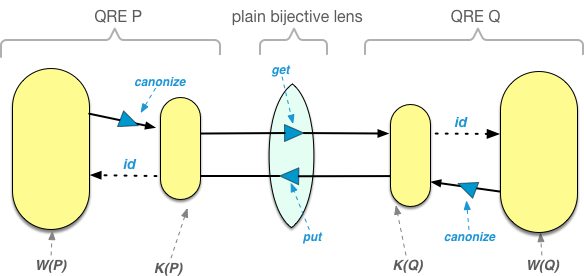
\includegraphics[width=0.7\textwidth]{QREs}
\caption{QRE lens from source $P$ to target $Q$.  $P$ and $Q$ are QREs, each
  consisting of a ``whole'' set ($W(P)$ and $W(Q)$) and a ``kernel'' part
  ($K(P)$ and $K(Q)$) Between the two kernels is a plain bijective lens.
  The \kw{get} function of the whole lens takes an argument from $W(P)$,
  applies the canonizer for $P$ to obtain a canonical representative in
  $K(P)$, then applies the \kw{get} of the plain lens, yielding an element
  of $K(Q)$, which is a subset of $W(Q)$.  The \kw{put} function does the
  reverse, mapping from $W(Q)$ to $K(P)$ (hence $W(P)$.  This lens is in
  normal form, with canonizers (specified by QREs) at the outer edges and an
  ordinary bijective lens in the center. }
\iflater
\saz{I think that this figure is a
  big improvement.  One tiny possible tweak: color the \kw{get} and \kw{put}
  keywords in the same color as in the text.}\bcp{Can do, if we keep the
  color in the text :-).  How are we going to decide about that?}\saz{Vote?}
\fi
\label{fig:attheedges}
\end{figure}
Every QRE lens $q$ has a type $P \Leftrightarrow Q$ where $P$ and $Q$
are QREs. In the {\em get} direction, a QRE lens $q: P \Leftrightarrow Q$ uses
the source QRE $P$ to compute a canonical representative for the data modulo
the equivalence relation defined by $P$ and then applies the \kw{get} function
of a bijective string lens $\ell$ to this representative. In the {\em put}
direction, $q$ operates similarly, but using the QRE $Q$ and the $\lput$
function of $\ell$.

Because the QREs $P$ and $Q$ determine the internal formats for data after
canonization, and because the algorithm for synthesizing bijective string
lenses is directed by these formats, $P$ and $Q$ are all that is required to
synthesize QRE lenses end-to-end. 

However, our requirement that canonizers appear only at the edges
raises a key technical question: Are we limiting the expressiveness of
our transformations by demanding all programs fit into this normal
form?  It turns out that we are not---any lens that uses canonizers
internally can be transformed into a lens that uses canonizers only at
the edges. The main technical contribution of this paper
(Theorem~\ref{normal form})
is a proof of this fact.
This technical result justifies 
using synthesis to produce QRE lenses instead of manually writing
them,
which can lead to substantial savings in program complexity.
For instance, after defining the \bibtex{} and EndNote QREs and
binding them to the variables \cd{bibtex} and \cd{endnote} respectively, then
all of the code in Figure~\ref{fig:example-lens} may be replaced by a single call
to the synthesis prodedure:
\begin{lstlisting}
let bib_to_end : bibtex $\Leftrightarrow$ endnote =
synth bibtex $\Leftrightarrow$ endnote using {(bib_example, end_example)}
\end{lstlisting}
\noindent 
Here, the generated quotient lens synchronizes \cd{bibtex} and
\cd{endnote} formats, using \cd{bib_example} and \cd{end_example} (the two
concrete example strings given at the beginning of this section) to
disambiguate. In addition, and as we saw earlier with the definition of
\cd{c_to_s}, the synthesis procedure itself can be used to create lenses that
are in turn used to define other QREs.  The ability to interleave QRE
specification with QRE lens synthesis yields a powerful and flexible way of
creating bidirectional transformations.

\section{Quotient Regular Expressions}
\label{QRE}
A Quotient Regular Expression (or QRE) is a regular expression $R$ augmented
with syntax that expresses an equivalence relation on the language of $R$. This
section formalizes the set of QRE combinators that we introduced informally
in \cref{sec:example}.

\subsection{Syntax and Semantics of QREs}
Formally, the language of Quotient Regular Expressions (QREs) is given by the
following grammar,
\begin{align*}
Q := \; & \normalize{R_1}{R_2}{f} \bsep{} \id(R) \bsep \collapse{R}{s} \bsep
\squash{Q_1}{Q_2}{f} \\ | \; & \perm{Q_1, \ldots, Q_n}{Q} \bsep Q_1 \semicolon
Q_2 \bsep Q_1 \cdot Q_2 \bsep (Q_1 \sep Q_2) \bsep Q^*
\end{align*}
where $Q$ ranges over QREs, 
$R$ ranges over regular expressions, 
$f$ ranges over functions between regular languages, and 
$s$ ranges over character strings.

Using the conventional notation that $\mathcal{L}(R)$ is the language accepted
by the regular expression $R$, each QRE $Q$ yields four semantic
objects:

\begin{tabular}{rl}
  $W(Q)$       & A regular expression, denoting the ``whole'' of $Q$\\
  $\eqrel{Q}$  & An equivalence relation on $\mathcal{L}(W(Q))$\\
  $K(Q)$       & A regular expression, denoting the ``kernel'' of $Q$, such that
                  $\mathcal{L}(K(Q))$ forms a \\
               & complete set of representatives for $\eqrel{Q}$ \\
  $\canonize(Q)$ & 
  A ``canonizing'' function. Given any $w \in \mathcal{L}(W(Q))$,
  $\canonize(Q)(w)$ \\ & is the unique $k$ in $\mathcal{L}(K(Q))$ such
  that $k \eqrel{Q} w$.
\end{tabular}
  % of type $\mathcal{L}(W(Q)) \longrightarrow \mathcal{L}(K(Q))$  which

\noindent
Intuitivley, $W(Q)$ is the regular expression representing the
external format, while $K(Q)$ is the regular expression representing
the internal format.  The equivalence relation $\eqrel{Q}$ groups
together elements in the language of $W(Q)$ that contain the same
essential information.  The function $\canonize(Q)$ picks the
representative element from each of the resulting equivalence classes.

The well-formedness constraints for QREs ensure that these four semantic
objects fit together to form a coherent quotient $W(Q)/\eqrel{Q}$ whose
equivalence classes are determined by $\canonize(Q)$.

\subsection{The \kw{normalize} Combinator}

The relationship among the semantic objects of a QRE can be understood in terms
of the combinator \normalize{R_1}{R_2}{f}, which expresses each of these pieces
explicitly.  Its whole language is just $R_1$, its kernel language is just
$R_2$, and its canonizer is just $f$; 
its equivalence relation $\equiv$ is
determined by the fibres of $f$, so we have
$s_1 \equiv s_2 \Leftrightarrow f(s_1) = f(s_2)$ for $s_1$ and $s_2$
in $\mathcal{L}(R_1)$.

These components form a coherent quotient language when the canonization
function $f$ is surjective and idempotent (intuitively, $f$ picks out a unique
representative for each equivalence class).  We also require that the kernel
language be a subset of the whole language, which enables QRE composition.
These considerations lead to the following well-formedness rule.

\begin{prooftree}
\AxiomC{$\mathcal{L}(R_2) \subseteq \mathcal{L}(R_1)$}
\AxiomC{$f : \mathcal{L}(R_1) \longrightarrow \mathcal{L}(R_2)$}
\AxiomC{$f$ is surjective}
\AxiomC{$f = f^2$}
\RightLabel{(Normalize)}
\QuaternaryInfC{$\wf{\normalize{R_1}{R_2}{f}}$}
\end{prooftree}

Semantically, the \kw{normalize} QRE is universal---each of the other
combinators $Q$ is equivalent to $\normalize{W(Q)}{K(Q)}{f}$ for some
surjective, idempotent function 
$f : \mathcal{L}(W(Q)) \longrightarrow \mathcal{L}(K(Q))$.  
However,
verifying that a canonization
function $f$ is surjective and idempotent is in general undecidable.
Consequently, a programmer wishing to use \kw{normalize} must
discharge strong proof obligations, which is cumbersome in
practice.\footnote{In our implementation we allow a programmer to
use \kw{normalize} at their own risk without checking these side
conditions as an ``escape hatch'' for the case when other QRE
combinators are insufficient.}

The remaining QRE combinators, which we discuss next, provide simpler, more
compositional ways of building canonizers that meet these requirements by
construction.  Nevertheless, the \kw{normalize} combinator provides a useful
guide in the design of these combinators because it gives a sufficient condition
for the well-formedness of any potential QREs.

% particularly with respect to the strategy for synthesizing quotient
% lenses (See Section~\ref{synth}), so we use it to guide the design of
% our QRE remaining combinators, which we discuss next.

% ; this is the second
% property that distinguishes the \kw{normalize} combinator from the other QREs.
% The \kw{normalize} combinator is special in two main ways, the first of 
% which has to do with the premises in its inference rule:


\subsection{QRE Combinator Semantics}

Figure~\ref{fig:wk} gives the inductive definitions of the whole and
kernel languages $W(Q)$ and $K(Q)$ for all of the QRE combinators.
\begin{figure}[t]
\centering
\[
\begin{array}{l@{\quad\quad}l@{\quad\quad}l}

Q & W(Q) & K(Q) \\ \hline
\id(R) & R & R \\
\collapse{R}{s} & R & s \\
\squash{Q_1}{Q_2}{f} & W(Q_1) \sep W(Q_2) & K(Q_2) \\
\normalize{R_1}{R_2}{f} & R_1 & R_2 \\
Q_1 \; ; \; Q_2 & W(Q_1) & K(Q_2) \\
Q_1 \cdot\; Q_2 & W(Q_1) \cdot W(Q_2) & K(Q_1) \cdot K(Q_2) \\
Q_1 \sep \; Q_2 & W(Q_1) \sep W(Q_2) & K(Q_1) \sep K(Q_2) \\
Q^* & W(Q)^* & K(Q)^* \\
\end{array}
\]
\[
\begin{array}{r@{\quad}l}
W( \perm{Q_1, \ldots, Q_n}{Q} ) = &
\bigcup \limits_{\sigma \in S_n} W(Q_{\sigma(1)}) \cdot W(Q) \cdot \ldots \cdot
W(Q) \cdot W(Q_{\sigma(n)})\\
K( \perm{Q_1, \ldots, Q_n}{Q} ) = & K(Q_1) \cdot K(Q) \cdot \ldots \cdot K(Q)
\cdot K(Q_n)
\end{array}
\]
\caption{Whole and Kernel regular expressions for QRE combinators. 
In describing regular expressions, we use the notations $\sep$ and $\bigcup$ for
alternation, the notation $\cdot$ for concatenation, and the notation
$*$ for Kleene closure.  
We use the notation $S_n$ to denote the set of all permutations of the
numbers $1$ to $n$.
}
\label{fig:wk}
\end{figure}
The \kw{squash} and \kw{permutation} combinators have the two most
interesting definitions. If $Q = \squash{Q_1}{Q_2}{f}$, then the whole language
of $Q$ is $W(Q_1) \sep W(Q_2)$ because the \kw{squash} combinator
merges the whole language $W(Q_1)$ of $Q_1$ with the whole language $W(Q_2)$ of $Q_2$.
The function $f : \mathcal{L}(W(Q_1)) \longrightarrow \mathcal{L}(W(Q_2))$,
maps $\mathcal{L}(W(Q_1))$ into $\mathcal{L}(W(Q_2))$ using $f$ and then
canonizes $W(Q_2)$ into $K(Q_2)$ using $\canonize(Q_2)$.

For the $\perm{Q_1, \ldots, Q_n}{Q}$ combinator, the whole language is the
union of languages of the form $W(Q_{\sigma(1)}) \cdot W(Q) \cdot \ldots \cdot
W(Q) \cdot W(Q_{\sigma(n)})$ for any permutation $\sigma$ in $S_n$, where
$S_n$ is the set of all permutations of the numbers $1$ to $n$. Intuitively,
the \kw{permutation} combinator allows for the string to match any
permutation of the $Q_i$'s while preserving the separator $Q$ in
between each of the $Q_i$'s. The kernel of the \kw{permutation} combinator
is the language $K(Q_1) \cdot K(Q) \cdot \ldots \cdot K(Q) \cdot K(Q_n)$,
because the canonical permutation is the identity permuation, with each of the
parts of the input that match $Q_i$ and $Q$ canonized into $K(Q_i)$ and $K(Q)$
respectively.

Figure~\ref{fig:canonizers} gives the inductive definitions of the
$\canonize{}$ function for each QRE.
\begin{figure}[t]
\begin{center}
\[
\begin{array}{l@\quad l @\quad l}
\canonize(\id(R))(w) &=& w \\
\canonize(\collapse{R}{s})(w) &=& s\\[1ex]
\canonize(\squash{Q_1}{Q_2}{f})(w) &=&
\begin{cases}
\canonize(Q_1)(f(w)) & \text{if } w \in \mathcal{L}(W(Q_1))\\
\canonize(Q_2)(w) & \text{otherwise}
\end{cases}\\[3ex]
\canonize(\normalize{R_1}{R_2}{f})(w) &=& f(w)\\
\canonize(Q_1 \; ; \; Q_2)(w) &=& \canonize(Q_2)(\canonize(Q_1)(w))\\
\canonize(Q_1 \cdot Q_2)(w_1 \cdot w_2) &=& \canonize(Q_1)(w_1) \cdot \canonize(Q_2)(w_2)\\[1ex]
\canonize(Q_1 \sep Q_2)(w) &=&
\begin{cases}
\canonize(Q_1)(w) & \text{if } w \in \mathcal{L}(W(Q_1))\\
\canonize(Q_2)(w) & \text{if } w \in \mathcal{L}(W(Q_2))\\
\end{cases}\\[3ex]
\canonize(Q^*)(w_1 \cdot \ldots \cdot w_n) &=&
\begin{cases}
\epsilon & \text{if } n = 0\\
\canonize(Q)(w_1)\cdot \ldots \cdot \canonize(Q)(w_n) & \text{if } n > 0
\end{cases}
\\[2ex]
\multicolumn{3}{l}{\canonize(\perm{Q_1, \ldots, Q_n}{Q})(r_{\sigma(1)}
\cdot s_1 \cdot \ldots \cdot s_{n-1} \cdot r_{\sigma(n)})(w_{\sigma(1)} \cdot
s_1 \cdot \ldots \cdot s_{n-1} \cdot w_{\sigma(n)})}\\[.5ex]
\multicolumn{3}{l}{\ =\ \ \canonize(Q_1)(r_1)(w_1) \cdot \canonize(Q)(s_1)
\cdot \ldots \cdot \canonize(Q)(s_{n-1})\cdot\canonize(Q_n)(r_n)(w_n)}
\end{array}
\]
\end{center}
\caption{QRE canonizers.  Here we assume that the input $w$ to the canonizers
  has been partitioned in the unique way guaranteed to exist by the lens unambiguity conditions.}
\label{fig:canonizers}
\end{figure}
The \kw{permutation} combinator gives rise to the most interesting
definition:
\[
\begin{array}{l}
\canonize(\perm{Q_1, \ldots, Q_n}{Q})(r_{\sigma(1)}
\cdot s_1 \cdot \ldots \cdot s_{n-1} \cdot r_{\sigma(n)})(w_{\sigma(1)} \cdot s_1
  \cdot \ldots \cdot s_{n-1} \cdot w_{\sigma(n)})\\[.5ex]
\ =\ \ \canonize(Q_1)(r_1)(w_1) \cdot \canonize(Q)(s_1) \cdot \ldots \cdot
\canonize(Q)(s_{n-1})\cdot\canonize(Q_n)(r_n)(w_n)
\end{array}
\]
\noindent 
which places the strings that match $Q_i$ and $Q$ according to the
canonical permutation (i.e., the identity permutation) before applying
the canonizers $\canonize(Q_i)$ and $\canonize(Q)$, respectively.

Finally, Figure ~\ref{fig:relations} gives the inductive definition of the
equivalence relation $\eqrel{Q}$, which is the set-theoretic semantics
of a QRE $Q$ as an equivalence relation on the regular language $W(Q)$.

\begin{figure}[t]
\centering
\[
\begin{array}{l@{}l@{\ \ }l}
w \; \equiv_{\normalize{R_1}{R_2}{f}} \; w' &\iff&
f(w)=f(w') \\
w \; \equiv_{\id(R)} \; w' &\iff& w = w' \\
w \; \equiv_{\collapse{R}{s}} \; w' &\iff& \mathit{True} \\ % \text{for all }w, w'\\
w \; \equiv_{\squash{Q_1}{Q_2}{f}} \; w' &\iff& f(w) \equiv_{Q_2} w'
\text{ or } w \equiv_{Q_2} w' \\
w \; \equiv_{Q_1 \; ; \; Q_2} \; w' &\iff& \exists k, k' \in
\mathcal{L}(K(Q_2)) \text{ such that } w \; \equiv_{Q_1} \; k, \; w' \;
\equiv_{Q_1} \; k', \text{ and } k \; \equiv_{Q_2} \; k'\\
w \; \equiv_{Q_1 \cdot Q_2} \; w'  &\iff& w = r_1
\cdot r_2, \; w' = {r'}_1 \cdot {r'}_2 \text{ with } r_1 \; \equiv_{Q_1}
\; {r'}_1, \; r_2 \; \equiv{Q_n} \; {r'}_2\\
w \; \equiv_{Q_1 \sep Q_2} \; w' &\iff& w \; \equiv_{Q_1} \; w'
\text{ or } \; w \; \equiv_{Q_2} \; w'\\
w \; \equiv_{Q^*} \; w' &\iff& w = r_1 \cdot \ldots \cdot r_n, \; w'
= {r'}_1 \cdot \ldots \cdot {r'}_n \text{ and } r_i \equiv_{Q} \; {r'}_i
\\
w \; \equiv_{\perm{Q_1, \ldots, Q_n}{Q}} \; w' &\iff& w = r_{\sigma(1)}
\cdot s_1 \cdot \ldots \cdot s_{n-1} \cdot r_{\sigma(n)}, \;
w' = {r'}_{\theta(1)} \cdot s'_1 \cdot \ldots \cdot s'_{n-1}
\cdot {r'}_{\theta(n)} \\
& & \text{for some } \sigma, \theta \in S_n, \text{ with } r_i \;
\equiv_{q_i} \; r'_i \text{ and } s_k \; \equiv_{Q} \; s'_{k}
\end{array}
\]
\caption{QRE Equivalence Relations}
\label{fig:relations}
\end{figure}
\subsection{Ambiguity and Well-Formed QREs}
\label{subsec:well-formed-qres}

To ensure that regular combinations of QREs are well-formed, we need
to enforce a variety of {\em unambiguity} constraints.  
Specifically, when applying regular combinators to QREs $Q_1$ and $Q_2$, we require that
if a string $s$ matches any of the regular expressions $W(Q_1) \cdot W(Q_2)$,
\quad $W(Q_1) \sep W(Q_2)$, \quad $W(Q_1)^*$, \quad $K(Q_1) \cdot K(Q_2)$,
\quad $K(Q_1) \sep K(Q_2)$, \quad $K(Q_1)^*$, then $s$ matches that regular
expression in only one way.
Formally, we say that regular expressions $R$ and $S$ are
\textit{unambiguosly concatenable}, written $R \cdot^! S$ if for all strings
$r, r' \in \mathcal{L}(R)$ and $s, s' \in \mathcal{L}(S)$, if $r \cdot s = r'
\cdot s'$, then $r = r'$ and $s = s'$. We say that a regular expression $R$ is
\textit{unambiguosly iterable}, written $R^{*!}$ if for all strings $r_1,
\ldots, r_m$ and $r'_1, \ldots, r'_n \in \mathcal{L}(R)$, if $r_1 \cdot \ldots
\cdot r_m = r'_1 \cdot \ldots \cdot r'_n$, then $m = n$ and $r_i = r'_i$. We say
that a regular expression $R$ is \textit{strongly unambiguous}\cite{Sippu1988}
if and only if (1) $R = \varnothing$, or (2) $R = S_1 \cdot S_2$ with $S_1,
S_2$ strongly unambiguous and $S_1 \cdot^! S_n$, or (3) $R = S_1 \sep S_2$ with
$S_1, S_2$ strongly unambiguous and $\mathcal{L}(S_1) \cap \mathcal{L}(S_2) =
\varnothing$, or (4) $R = S^*$ with $S$ strongly unambiguous and $S^{*!}$.

These unambiguity constraints can be a little fiddly in practice. As a simple example of this, consider writing a regular expression for comma-separated lists of strings. Our first impulse might be to write it as,
\begin{lstlisting}
CSL = anychar+ . ("," . anychar+)*
\end{lstlisting}
(where . is concatenation), but this regular expression is ambiguous, as \lstinline|anychar| is a big union of a of single characters including comma.

While the unambiguity constraints consequently appear to compromise compositionality of QREs, they can usually be circumvented by making a small changes to the offending regular expression: for instance, in the preceding example, then we need to write,
\begin{lstlisting}
CSL = anycharexceptcomma+ . ("," . anycharexceptcomma+)*
\end{lstlisting}
(assuming \lstinline|anycharexceptcomma| denotes a big union of every single character string except comma). 

Unambiguity constraints are necessary because they ensure that the canonizing function of a QRE is well-defined.
For example, consider the QRE \lstinline|"a"$^*$ . (collapse "a"$^*$ $\to$ "a")|. The
behavior of this QRE is not well-defined since the string
\cd{"aaa"} can be canonized to any of \cd{"a"}, \cd{"aa"}, or \cd{"aaa"}
depending on how \cd{"aaa"} is parsed. The unambiguity constraints are also applied to the kernels of QREs since the underlying
bijective string lens of a QRE lens operates on kernels, and bijective string lenses
impose the same unambiguity restrictions so that they too are well defined as
functions.

\subsection{Well-formedness of QREs}

Figure~\ref{fig:qrerules} gives the inference rules for deriving well-formed
QREs.
\begin{figure}[tp!]
\begin{center}
\AxiomC{$R$ is strongly unambiguous}
\RightLabel{(Id)}
\UnaryInfC{$\wf{\kw{id}(R)}$}
\DisplayProof
\hskip 1.5em
\AxiomC{$s \in \mathcal{L}(R)$}
\RightLabel{(Collapse)}
\UnaryInfC{$\wf{\collapse{R}{s}}$}
\DisplayProof
\hskip 1.5em
\end{center}

\begin{prooftree}
\AxiomC{$\wf{Q_i, Q}$}
\RightLabel{(Perm)}
\AxiomC{${\substack{\forall \sigma \neq \theta, \; W(Q_{\sigma(1)}) \cdot W(Q)
\cdot \ldots \cdot W(Q_{\sigma(n)})\\ \cap W(Q_{\theta(1)}) \cdot W(Q)
\cdot \ldots \cdot W(Q_{\theta(n)}) =\varnothing}}$}
\AxiomC{$K(Q_1) \cdot^! K(Q) \cdot^! \ldots \cdot^! K(Q) \cdot^! K(Q_n)$}
\TrinaryInfC{$\wf{\perm{Q_1, \ldots, Q_n}{Q}}$}
\end{prooftree}

\begin{center}
\AxiomC{$\wf{Q_1, Q_2}$}
\AxiomC{$\mathcal{L}(W(Q_1)) \cap \mathcal{L}(W(Q_2)) = \varnothing$}
\AxiomC{$f : \mathcal{L}(W(Q_1)) \longrightarrow \mathcal{L}(W(Q_2))$}
\RightLabel{(Squash)}
\TrinaryInfC{$\wf{\squash{Q_1}{Q_2}{f}}$}
\DisplayProof
\end{center}
\begin{center}

\begin{prooftree}
\AxiomC{$\mathcal{L}(R') \subseteq \mathcal{L}(R)$}
\AxiomC{$f : \mathcal{L}(R) \longrightarrow \mathcal{L}(R')$}
\AxiomC{$f$ is surjective}
\AxiomC{$f = f^2$}
\RightLabel{(Normalize)}
\QuaternaryInfC{$\wf{\normalize{R}{R'}{f}}$}
\end{prooftree}

\end{center}
\begin{center}
\AxiomC{$\wf{Q_1, Q_2}$}
\AxiomC{$K(Q_1) = W(Q_2)$}
\RightLabel{(Compose)}
\BinaryInfC{$\wf{Q_1 \; ; \; Q_2}$}
\DisplayProof
\hskip 1.5em
\AxiomC{$\wf{Q}$}
\AxiomC{$W(Q)^{*!}$}
\AxiomC{$K(Q)^{*!}$}
\RightLabel{(Star)}
\TrinaryInfC{$\wf{Q^*}$}
\DisplayProof
\end{center}
\begin{center}

\begin{center}
\AxiomC{$\wf{Q_1, Q_2}$}
\AxiomC{$W(Q_1) \cdot^! W(Q_2)$}
\AxiomC{$K(Q_1) \cdot^! K(Q_2)$}
\RightLabel{(Concat)}
\TrinaryInfC{$\wf{Q_1 \cdot Q_2}$}
\DisplayProof
\end{center}

\begin{center}
\AxiomC{$\wf{Q_1, Q_2}$}
\AxiomC{$W(Q_1) \cap W(Q_2) = \varnothing$}
\RightLabel{(Union)}
\BinaryInfC{$\wf{Q_1 \sep Q_2}$}
\DisplayProof
\
\end{center}
\end{center}
\caption{Well-formed QREs}
\label{fig:qrerules}
\end{figure}
The unambiguity conditions are pertinent when defining QREs using the
regular combinators. For example, the (Concat) inference rule 
says that the concatenation $Q_1 \cdot Q_2$ of QREs
$Q_1$ and $Q_2$ is well formed only if the concatentions of $W(Q_1)$
and $W(Q_2)$, and $K(Q_1)$ and $K(Q_2)$ are unambiguous.

The most complicated inference rule is the (Perm) rule for the
permutation combinator. The second hypothesis for the
Perm rule says that for any two different permutations $\sigma$
and $\theta$, the languages $W(Q_{\sigma(1)}) \cdot W(Q) \cdot \ldots \cdot
W(Q_{\sigma(n)})$ and $W(Q_{\theta(1)}) \cdot W(Q) \cdot \ldots \cdot
W(Q_{\theta(n)})$ must be disjoint. This restriction is important
because an input string could match any
of the regular expressions $W(Q_{\theta(1)}) \cdot
W(Q) \cdot \ldots \cdot W(Q_{\theta(n)})$ for some permutation $\theta$, so we
must require that all of them be disjoint.
%
The third hypothesis says that the regular expression $K(Q_1) \cdot K(Q)
\cdot \ldots \cdot K(Q) \cdot K(Q_n)$ must be unambiguous. This
restriction arises because the
underlying lens that maps to or from a \kw{perm} QRE operates on
the language $K(Q_1) \cdot K(Q) \cdot \ldots \cdot K(Q) \cdot K(Q_n)$, 
the kernel of the \kw{perm} QRE. The underlying
lens requires that the source and target regular expressions be
unambiguous so that the lens can match strings uniquely.


\section{QRE Lenses}
\label{QRE-lenses}
As we have seen, QREs express a broad class of equivalence relations
directly on regular languages. QREs are therefore a good \textit{specification}
language for quotient lenses. In this section we introduce \textit{QRE Lenses},
a class of quotient lenses that map between data that is specified using QREs.

Recall that given regular expressions $R, S$ and equivalence relations
$\equiv_R$ and $\equiv_S$ defined on $\mathcal{L}(R)$ and $\mathcal{L}(S)$, a
{\em bijective quotient lens} $q : R /{\equiv_R} \Leftrightarrow S/{\equiv_S}$
is a pair of functions $q.\get : \mathcal{L}(R) \longrightarrow \mathcal{L}(S)$
and $q.\lput : \mathcal{L}(S) \longrightarrow \mathcal{L}(R)$ such that for all
$r \in \mathcal{L}(R)$ and $s \in \mathcal{L}(S)$, we have $q.\lput(q_1.\get(r))
\equiv_R r$ and $q.\get(q_1.\lput(s)) \equiv_R s$. Moreover, if $r \equiv_R
r'$, then $q.\get(r) = q.\get(r')$, and if $s \equiv_S s'$, then $q.\lput(s) =
q.\lput(s')$. In words, a bijective quotient lens $q$ from $R$ to $S$ modulo
$\equiv_R$ and $\equiv_S$ is a pair of functions $q.\get$ and $q.\lput$ such
that $q.\get$ respects $\equiv_R$ and $q.\lput$ respects $\equiv_S$, and such
that the {\em get} and {\em put} functions lifted to $\mathcal{L}(R)/{\equiv_R}$
and $\mathcal{L}(S)/{\equiv_S}$ are mutual inverses. These laws are similar
bijective lens laws \cref{bijectivelenslaws}, except that the equality
restrictions in the bijective lens laws are loosened to allow for equivalence
relations. Also, the condition that $r \equiv_R r'$ implies $q.\get(r) =
q.\get(r')$ ensures that the \kw{get} function induced on the equivalence
classes of $\equiv_R$ is well-defined, and similarly for the \kw{put}
function.

Having identified QREs as a natural way of specifing equivalence relations on
regular expressions, a natural next step in defining quotient lenses is to map
between two QREs via a bijection between their kernels; indeed, this approach
is the one we adopt in defining {\em QRE lenses}.
More concretely, to define a language of QRE lenses, we
(1) define a language of bijections (Section \ref{subsec:bijective-lenses}),
(2) add quotients by allowing canonizers to be prepended or postpended
to bijections, and 
(3) allow composition of such quotient lenses via the
regular operators and functional composition
(Sections \ref{subsec:qre-lenses-syntax} and \ref{subsec:qre-lenses-semantics}).

However, we also have a secondary objective, which is to support lens
synthesis. When provided with QREs describing the source and target
languages, we would like to be able to generate quotient lenses
automatically. One way to achieve that goal is to generate canonizers
$\canonize(Q_1)$ and $\canonize(Q_2)$ from QREs $Q_1$ and $Q_2$ and
then to synthesize bijective lenses between the kernel languages for
$Q_1$ and $Q_2$.
Unfortunately, the composition of two such quotient lenses does not have 
the form of a bijective lens with canonizers at the edges. Hence, an important
technical question is whether we give up expressiveness if we restrict
ourselves to this form. 
Fortunately, we can show that there is no loss of expressiveness if
the bijections used to define QRE lenses are derived with a particular
set of combinators.  We describe these combinators next.

\subsection{Bijective String Lenses}
\label{subsec:bijective-lenses}
We define the set of \textit{bijective string lenses} to be the set of
bijections between regular languages constructed using the following
combinators,
$$\ell := \id(R) \sep \const(s, t) \sep  \swap(\ell_1, \ell_2)
\sep \ell_1 \cdot \ell_2 \; |  \; (\ell_1 \sep \ell_2) \sep \ell^* \; | \;
\ell_1 \; ; \;  \ell_2$$
where $R$ ranges over regular expressions and $s$ ranges over character strings.

The $\mathit{\const}(s, t)$ lens replaces the string $s$ with $t$ in the source
data in the forward direction, and $t$ with $s$ in the target data in the
backward direction, while $\kw{id}(R)$ applies the identity function to the
source and target  in $\mathcal{L}(R)$ in both directions. The composition lens
$\ell_1 \; ; \; \ell_2$ applies $\ell_1$ followed by then $\ell_2$ to the
source in the forward direction, and applies $\ell_2$ followed by $\ell_1$ to
the target in the backward direction. The lens $\ell_1 \cdot \ell_2$ first
splits the string $s$ into $s_1$ and $s_2$, applies $\ell_1$ and $\ell_2$ to
$s_1$ and $s_2$ to get $t_1$ and $t_2$ respectively, then concatenates $t_1$
and $t_2$ and returns $t_1 \cdot t_2$ as the final result in the forward
direction. $\ell_1 \cdot \ell_2$ operates similarly in the backward direction,
but with $s, s_1$ and $s_2$ substituted for $t, t_1$ and $t_2$. The
$\swap(\ell_1, \ell_2)$ lens operates like $\ell_1 \cdot \ell_2$,
except that it swaps $t_1$ and $t_2$ before concatenating the two for a final
result of $t_2 \cdot t_1$ in the forward direction. In the backward direction,
$\swap(\ell_1, \ell_2)$ first undoes the \swap, then behaves like
the concatenation lens. The $\ell_1 \; | \; \ell_2$ lens chooses to apply
$\ell_1$ or $\ell_2$ depending on whether the source (resp. target) data is
matched by $\ell_1$ or $\ell_2$ in the forward (resp. backward direction). The
$\ell^*$ lens splits the string $s$ into strings $s_1, \ldots, s_n$, applies
$\ell_1$ to each $s_i$ to obtain $t_i$, and then concatenates each of the $t_i$'s
for a final result of $t_1 \cdot \ldots \cdot t_n$ in the forward direction.
The iteration lens $\ell^*$ operates similarly in the backward direction, but
with $s$ and $s_i$ substituted for $t$ and $t_i$.

The denotation of a lens $\ell_1$ is $\llbracket \ell_1 \rrbracket \subseteq
\mathit{String} \times \mathit{String}$. If $(s_1, s_2) \in \llbracket \ell_1
\rrbracket$, then $\ell_1$ maps between $s_1$ and $s_2$.
\begin{align*}
\llbracket \id(R) \rrbracket &= \{(r, r) \sep r \in \mathcal{L}(R)\}\\
\llbracket \const(r, s) \rrbracket &= \{(r, s)\}\\
\llbracket \swap(\ell_1, \ell_2) \rrbracket &= \{(s \cdot t, t' \cdot s') \sep
(s, s') \in \llbracket \ell_1 \rrbracket \text{ and } (t, t') \in \llbracket
\ell_2 \rrbracket\}\\
\llbracket \ell_1 \cdot \ell_2 \rrbracket &= \{(s \cdot t, s' \cdot t) \sep
(s, s') \in \llbracket \ell_1 \rrbracket \text{ and } (t, t') \in \llbracket
\ell_2 \rrbracket\}\\
\llbracket \ell_1 \sep \ell_2 \rrbracket &= \{(s \cdot t) \sep
(s, t) \in \llbracket \ell_1 \rrbracket \text{ or } (s, t) \in \llbracket
\ell_2 \rrbracket\}\\
\llbracket \ell^* \rrbracket &= \{(s_1 \cdot \ldots \cdot s_n, t_1 \cdot \ldots
\cdot t_n) \sep (s_i, t_i) \in \llbracket \ell \rrbracket \text{ for } 1
\leq i \leq n\}\\
\llbracket \ell_1 \; ; \; \ell_2 \rrbracket &= \{(r, t) \sep \text{there exists }s
\text{ such that } (r, s) \in \llbracket \ell_1 \rrbracket \text{ and } (s, t)
\in \llbracket \ell_2 \rrbracket\}
\end{align*}

Each bijective string lens $\ell$ has a type $\ell : R \Leftrightarrow S$ where
$R$ and $S$ are regular expressions. If $\ell : R \Leftrightarrow S$, then the
source language of $\ell$ is $\mathcal{L}(R)$ and the target language of $\ell$
is $\mathcal{L}(S)$. IThe final rule in the figure deserves special attention.
It states that a lens $\ell : R \Leftrightarrow S$ can also be considered to be
of type $\ell : R' \Leftrightarrow S'$ provided that $R$ (resp. $S$) can be
proven to be equivalent to $R'$ (resp. $S$) from the star-semiring axioms
(associativity and commutativity of | and $\cdot$, identity of the empty string
$\epsilon$, distibutivity of $\cdot$ over |, annihilative property of
$\varnothing$ with respect to $\cdot$, and that $R^* = \epsilon \; | \; R \cdot
R^* = \epsilon \; | \; R^* \cdot R$ for all $R$):

\begin{prooftree}
\AxiomC{$\ell_1 : R \Leftrightarrow S$}
\AxiomC{$R \equiv^s R'$}
\AxiomC{$S \equiv^s S'$}
\TrinaryInfC{$\ell_1 : R' \Leftrightarrow S'$}
\end{prooftree}

\noindent
This rule makes it significantly more difficult to synthesize a bijective lens
from its type.

\begin{figure}[t]
\begin{center}
\AxiomC{$s_1 \in \Sigma^*$}
\AxiomC{$s_2 \in \Sigma^*$}
\BinaryInfC{$\mathit{\const} \; (s_1, s_t): s_1 \Leftrightarrow s_2$}
\DisplayProof
\hskip 1.5em
\AxiomC{$R$ is strongly unambiguous}
\UnaryInfC{$\kw{id}(R): R \Leftrightarrow R$}
\DisplayProof
\end{center}

\begin{center}
\AxiomC{$\substack{\ell_1 : R_1 \Leftrightarrow S_1 \\ \ell_2 : R_2
\Leftrightarrow S_2}$}
\AxiomC{$\substack{R_1 \cdot^! R_2 \\S_1 \cdot^! S_2 }$}
\BinaryInfC{$\ell_1 \cdot \ell_2: R_1 \cdot R_2 \Leftrightarrow S_1 \cdot
S_2$}
\DisplayProof
\hskip 1.5em
\AxiomC{$\substack{\ell_1 : R_1 \Leftrightarrow S_1 \\ \ell_2 : R_2
\Leftrightarrow S_2}$}
\AxiomC{$\substack{R_1 \cdot^! R_2 \\ S_2 \cdot^! S_1}$}
\BinaryInfC{$\mathit{\swap} \; (\ell_1, \ell_2): R_1 \cdot R_2
\Leftrightarrow S_2 \cdot S_1$}
\DisplayProof
\end{center}

\begin{center}
\AxiomC{$\ell_1 : R_1 \Leftrightarrow R_2$}
\AxiomC{$\ell_2 : R_2 \Leftrightarrow R_3$}
\BinaryInfC{$\ell_1 \; ; \; \ell_2: R_1 \Leftrightarrow R_3$}
\DisplayProof
\hskip 1.5em
\AxiomC{$\substack{\ell_1 : R_1 \Leftrightarrow S_1 \\ \ell_2 : R_2
\Leftrightarrow S_2}$}
\AxiomC{$\substack{\mathcal{L}(R_1) \cap \mathcal{L}(R_2) =
\varnothing \\ \mathcal{L}(S_1) \cap \mathcal{L}(S_2) = \varnothing}$}
\BinaryInfC{$\ell_1 \sep \ell_2: R_1 \sep R_2 \Leftrightarrow S_1 \sep S_2$}
\DisplayProof
\end{center}

\begin{center}
\AxiomC{$\ell : R \Leftrightarrow S$}
\AxiomC{$R^{*!}$}
\AxiomC{$S^{*!}$}
\TrinaryInfC{$\ell^*: R \Leftrightarrow S$}
\DisplayProof
\hskip 1.5em
\AxiomC{$\ell : R \Leftrightarrow S$}
\AxiomC{$R \equiv^s R'$}
\AxiomC{$S \equiv^s S'$}
\TrinaryInfC{$\ell : R' \Leftrightarrow S'$}
\DisplayProof
\end{center}
\caption{Bijective String Lens Typing Rules}
\label{fig:lensrules}
\end{figure}

\subsection{Syntax of QRE Lenses}
\label{subsec:qre-lenses-syntax}
Having given a brief overview of the class of bijective string lenses, we now
introduce the class of QRE lenses. The language of QRE lenses is given by
following grammar,
$$ q := \lift(\ell) \sep  q_1 \cdot q_2 \sep \swap(q_1, q_2) \sep (q_1 \sep q_2)
\sep q^* \sep q_1 \; ; \; q_2 \sep \lquot(q, \ell) \sep \rquot(\ell, q)$$
where $\ell$ ranges over bijective lenses.

Other than the \kw{lift} combinator which allows a bijective lens to be
treated as a quotient lens, the QRE lens combinators are the same as the
bijective string lens combinators but with two extra combinators where
quotienting actually occurs: the $\lquot$ and $\rquot$ combinators. The
$\lquot(Q, q)$ combinator takes a quotient lens $q$ and quotients the source
data using $Q$, assuming that the source data forms a complete set of
representatives for the equivalence relation $\eqrel{Q}$. The $\lquot(q, Q)$
combinator does the same but on the target data.

For example, recall that in the \bibtex{} to EndNote transformation, we had the
QREs \cd{bibtex} and \cd{endnote} and the bijective lens \cd{bib_to_end}
that maps between 
\cd{bibtex} and \cd{endnote}. The quotient lens that maps between
\cd{bibtex} and \cd{endnote} is then given by the following QRE lens:

\begin{lstlisting}
let bib_to_end_q : bibtex $\Leftrightarrow$ endnote =  rquot (lquot(bibtex, bib_to_end), endnote)
\end{lstlisting}

\subsection{Semantics of QRE Lenses}
\label{subsec:qre-lenses-semantics}
Each QRE lens $q$ has a type $q : Q_1 \Leftrightarrow Q_2$ where $Q_1, Q_2$ are
QREs. If $q : Q_1 \Leftrightarrow Q_2$, then the source format is described by
$W(Q_1)$ and the canonical set of representative for the source data is
described by $K(Q_1)$.
Similarly, the target format is described by $W(Q_2)$ and the canonical set of
representatives for the target data is described by $K(Q_2)$. The underlying
lens of $q$ is a bijective lens $\ell : K(Q_1) \Leftrightarrow K(Q_2)$.

The denotation $\llbracket q \rrbracket$ of a QRE lens $q : Q_1 \Leftrightarrow
Q_2$ is a quotient lens $\llbracket q \rrbracket : W(Q_1)/{\eqrel{Q_1}}
\Longleftrightarrow W(Q_2)/{\eqrel{Q_2}}$. The typing rules and denotation of
QRE lenses are given in Figure~\ref{fig:qlenssemantics}.
\begin{figure}[ht]
\centering
\[
\begin{array}[b]{l@{\qquad}l}
\RuleSide{\ell : R \Leftrightarrow S}{\kw{lift}(\ell): id(R) \Leftrightarrow
id(S)}{\mathit{(Lift)}} &
\begin{array}[b]{r@{\ }c@{\ }l}
\llbracket \kw{lift}(\ell) \rrbracket.\get &=&  \llbracket \ell \rrbracket\\
\llbracket \kw{lift}(\ell) \rrbracket.\lput &=& \llbracket \ell \rrbracket^{-1}
\end{array}
\end{array}
\]

\[
\begin{array}[b]{c@{\qquad}c}
\RuleSide{q : Q_2  \Leftrightarrow Q_3 &
\wf{Q_1} &
K(Q_1) = W(Q_2)}
{\lquot(Q_1, q): Q_1 \; ; \; Q_2 \Leftrightarrow Q_3}{\mathit(Lquot)} &
\begin{array}[b]{r@{\ }c@{\ }l}
\llbracket \lquot(Q_1, q) \rrbracket.\get  &=& \llbracket q
\rrbracket.\get \circ \canonize(Q_1)\\
\llbracket \lquot(Q_1, q) \rrbracket.\lput &=& \llbracket q
\rrbracket.\lput
\end{array}
\end{array}
\]

\[
\begin{array}[b]{c@{\qquad}c}
\RuleSide{q : Q_1 \Leftrightarrow Q_3 & \wf{Q_3} & W(Q_3) = K(Q_2)}
{\rquot(q, Q_1):Q_1 \Leftrightarrow Q_2 \; ; \; Q_3}{\mathit{(Rquot)}} &
\begin{array}[b]{r@{\ }c@{\ }l}
\llbracket \rquot(q, Q_1) \rrbracket.\get  &=& \llbracket q
\rrbracket.\get\\
\llbracket \rquot(q, Q_1) \rrbracket.\lput &=& \llbracket q
\rrbracket.\lput \circ \canonize(Q_3)
\end{array}
\end{array}
\]

\[
\begin{array}[b]{l@{\qquad}c}
\RuleSide{q : Q_1 \Leftrightarrow Q_2 &
W(Q_1)^{*!},W(Q_2)^{*!} & K(Q_1)^{*!}, K(Q_2)^{*!}}
{{q}^* : {Q_1}^* \Leftrightarrow {Q_2}^*}{\mathit{(Star)}} &
\begin{array}[b]{r@{\ }c@{\ }l}
\llbracket {q}^* \rrbracket.\get  &=& (\llbracket q \rrbracket.\get)^*\\
\llbracket {q}^* \rrbracket.\lput &=& (\llbracket q \rrbracket.\get)^*
\end{array}
\end{array}
\]

\[
\begin{array}[b]{l@{\qquad}c}
\RuleSide{\substack{q_1 : Q_1 \Leftrightarrow Q_3 \\ q_2 : Q_2 \Leftrightarrow
Q_4} & {\substack{W(Q_1) \cdot^! W(Q_2)\\ K(Q_1) \cdot^! K(Q_2)}}
& {\substack{W(Q_3) \cdot^! W(Q_4)\\ K(Q_3) \cdot^! K(Q_4)}}}
{q_1 \cdot q_2: Q_1 \cdot Q_2 \Leftrightarrow Q_3 \cdot Q_4}{\mathit{(Concat)}}
&
\begin{array}[b]{r@{\ }c@{\ }l}
\llbracket q_1 \cdot q_2 \rrbracket.\get  &=& \llbracket q_1 \rrbracket.\get
\cdot \llbracket q_2 \rrbracket.\get\\
\llbracket q_1 \cdot q_2\rrbracket.\lput &=& \llbracket q_1 \rrbracket.\lput
\cdot \llbracket q_2 \rrbracket.\lput
\end{array}
\end{array}
\]

\[
\begin{array}[b]{l@{\qquad}c}
\RuleSide{\substack{q_1 : Q_1 \Leftrightarrow Q_3 \\ q_2 : Q_2 \Leftrightarrow
Q_4} & {\substack{W(Q_1) \cdot^! W(Q_2)\\ K(Q_1) \cdot^! K(Q_2)}}
& {\substack{W(Q_4) \cdot^! W(Q_3)\\ K(Q_4) \cdot^! K(Q_3)}}}
{q= q_1 \cdot q_2: Q_1 \cdot Q_2 \Leftrightarrow Q_4 \cdot
Q_3}{\mathit{(Swap)}} &
\begin{array}[b]{r@{\ }c@{\ }l}
\llbracket q \rrbracket.\get(s_1 \cdot s_2)  &=& \llbracket q_2
\rrbracket.\get(s_2) \cdot \llbracket q_1 \rrbracket.\get(s_1)\\
\llbracket q \rrbracket.\lput(t_2 \cdot t_1) &=&
\llbracket q_1 \rrbracket.\lput(t_1) \cdot \llbracket q_2 \rrbracket.\lput(t_2)
\end{array}
\end{array}
\]

\[
\begin{array}[b]{l@{\qquad}c}
\RuleSide{\substack{q_1 : Q_1 \Leftrightarrow Q_3 \\ q_2 : Q_2 \Leftrightarrow
Q_4} & \substack{\mathcal{L}(W(Q_1)) \cap \mathcal{L}(W(Q_2)) = \varnothing
\\ \mathcal{L}(W(Q_3)) \cap \mathcal{L}(W(Q_4)) = \varnothing }}
{q_1 \sep q_2: (Q_1 \sep Q_2)\Leftrightarrow (Q_3 \sep Q_4)}{\mathit{(Or)}} &
\begin{array}[b]{r@{\ }c@{\ }l}
\llbracket q_1 \sep q_2 \rrbracket.\get(s) =
\begin{cases}
\llbracket q_1 \rrbracket.\get (s) & \text{if } s \in \mathcal{L}(W(Q_1))\\
\llbracket q_2 \rrbracket.\get (s) & \text{if } s \in \mathcal{L}(W(Q_2))\\
\end{cases}\\
\llbracket q_1 \sep q_2 \rrbracket.\lput(s) =
\begin{cases}
\llbracket q_1 \rrbracket.\lput (s) & \text{if } s \in \mathcal{L}(W(Q_3))\\
\llbracket q_2 \rrbracket.\lput (s) & \text{if } s \in \mathcal{L}(W(Q_4))\\
\end{cases}
\end{array}
\end{array}
\]

\begin{prooftree}
\AxiomC{$\substack{q_1 : Q_1 \Leftrightarrow Q_2 \\ q_2 : Q_3 \Leftrightarrow
Q_4}$}
\RightLabel{(Compose)}
\AxiomC{$\substack{\mathcal{L}(W(Q_2))= \mathcal{L}(W(Q_3)) \\ K(Q_2) \equiv^s
K(Q_3)}$}
\AxiomC{$\canonize(Q_2) = \canonize(Q_3)$}
\TrinaryInfC{$q_1 \; ; \; q_2: Q_1 \Leftrightarrow Q_4$}
\end{prooftree}
\begin{align*}
\llbracket q_1 \; ; \; q_2 \rrbracket.\get &= \llbracket q_2
\rrbracket.\get\circ \llbracket q_1 \rrbracket.\get\\
\llbracket q_1 \; ; \; q_2 \rrbracket.\lput &= \llbracket q_1 \rrbracket.\lput
\circ \llbracket q_2 \rrbracket.\lput
\end{align*}
\caption{Denotation and Typing Rules for QRE Lenses}
\label{fig:qlenssemantics}
\end{figure}
The trickiest typing rule is the typing rule for composition:

\begin{prooftree}
\AxiomC{$\substack{q_1 : Q_1 \Leftrightarrow Q_2 \\ q_2 : Q_3 \Leftrightarrow
Q_4}$}
\AxiomC{$\substack{\mathcal{L}(W(Q_2))= \mathcal{L}(W(Q_3)) \\ K(Q_2) \equiv^s
K(Q_3)}$}
\AxiomC{$\canonize(Q_2) = \canonize(Q_3)$}
\TrinaryInfC{$q_1 \; ; \; q_2: Q_1 \Leftrightarrow Q_4$}
\end{prooftree}

This rule essentially says that the composition $q_1 \; ; \; q_2$ is well
defined if and only if the intermediary QREs $Q_3$ and $Q_4$ define the same
equivalence relation on regular expressions that are equivalent modulo the
star-semiring axioms. (See~\cite[\S 4]{quotientlenses} for an example of what
goes wrong if this premise is dropped). The condition $\mathcal{L}(W(Q_2)) =
\mathcal{L}(W(Q_3))$ says that the intermediary language is the same on both
sides, while the condition $K(Q_2) \equiv^s K(Q_3)$ says that the kernel
regular expressions are equivalent modulo the star-semiring axioms. Finally,
the condition $\canonize(Q_2) = \canonize(Q_3)$ says that $Q_2$ and $Q_3$
define the same equivalence relation on $\mathcal{L}(W(Q_2))=
\mathcal{L}(W(Q_3))$.

Of course checking the condition $\canonize(Q_2) = \canonize(Q_3)$ is
undecidable in general; indeed the approach used to type quotient lenses in
Boomerang is to classify equivalences according to whether they are or are not
the equality relation. While this decision seemingly restricts the
power of composition in Boomerang significantly, the practice of writing
quotient lenses shows that this restriction is not overly restrictive. This is 
because most quotient lenses originate as lifted basic lenses, and
therefore have types whose equivalence relations are both equality, and further,
equality is preserved by many of the quotient lens combinators
~\cite{quotientlenses}. Foster et al also discuss a second possible approach to
typing quotient lenses, where equivalence relations are represented by rational
functions that induce them. While this second approach is more refined than the
first, Boomerang favours the first approach since the second appears to be too
expensive to be useful in practice. 

Thankfully, we do not face the issue of checking equivalence relation equality
in our work since our end goal is to synthesize lenses and not write them my
hand, so the programmer will never actually need to typecheck a functional
composition expression.

The semantics defined on QRE lenses imply the following theorem:
\begin{theorem}
If there is a derivation $q : Q_1 \Leftrightarrow Q_2$, then $\llbracket q
\rrbracket : W(Q_1)/{\eqrel{Q_1}} \Leftrightarrow W(Q_2)/{\eqrel{Q_2}}$ is a
well-defined quotient lens.
\end{theorem}
\subsection{Normal Forms of QRE Lenses}
Recall that our approach in defining QRE lenses is to have each QRE lens $q: Q_1
\Leftrightarrow Q_2$ be such that
\begin{align*}
\llbracket q \rrbracket.\get &= \ell \circ \canonize(Q_1)\\
\llbracket q \rrbracket.\lput &= \ell^{-1} \circ \canonize(Q_2)
\end{align*}
for some bijective lens $\ell$. In other words, each QRE lens is the same as a
bijective lens with canonizers at the edges. The following theorem,
which is the main technical contribution of this paper, confirms that this
indeed is the case:

\begin{theorem}\label{normal form}
If there is a derivation $q : Q_1 \Leftrightarrow Q_2$, then there exists a
bijective lens $\ell : K(Q_1) \Leftrightarrow K(Q_2)$ such that:
\begin{align*}
\llbracket q \rrbracket.\get &= \llbracket \ell \rrbracket\circ
\canonize(Q_1)\\
\llbracket q \rrbracket.\lput &= \llbracket \ell \rrbracket^{-1} \circ
\canonize(Q_2)
\end{align*}
\end{theorem}
\begin{proof}
The proof follows by induction on the derivation of $q : c \Leftrightarrow c$.
The most interesting part of the proof is the case for functional composition
as we must demonstrate that it is possible to eliminate the canonizers in the
middle of the term.

The derivation rule and denotation for composition are as follows:
\begin{prooftree}
\AxiomC{$\substack{q_1 : Q_1 \Leftrightarrow Q_2 \\ q_2 : Q_3 \Leftrightarrow
Q_4}$}
\AxiomC{$\substack{\mathcal{L}(W(Q_2))= \mathcal{L}(W(Q_3)) \\ K(Q_2) \equiv
K(Q_3)}$}
\AxiomC{$\canonize(Q_2) = \canonize(Q_3)$}
\TrinaryInfC{$q_1 \; ; \; q_2: Q_1 \Leftrightarrow Q_4$}
\end{prooftree}

\begin{align*}
\llbracket q_1 \; ; \; q_2 \rrbracket.\get &= \llbracket q_2 \rrbracket.\get\circ
\llbracket q_1 \rrbracket.\get\\
\llbracket q_1 \; ; \; q_2 \rrbracket.\lput &= \llbracket q_1 \rrbracket.\lput
\circ \llbracket q_2 \rrbracket.\lput
\end{align*}

By the induction hypothesis, there exist bijective lenses,
$\ell_1 : K(Q_1) \Leftrightarrow K(Q_2)$ and $\ell_2 : K(Q_3) \Leftrightarrow
K(Q_4)$ such that:
\begin{center}
\begin{tabular}{l l}
$\llbracket q_1 \rrbracket.\get = \llbracket \ell_1 \rrbracket \circ
\canonize(Q_1)$ & $\llbracket q_2 \rrbracket.\get = \llbracket \ell_2
\rrbracket \circ \canonize(Q_3)$ \\
$\llbracket q_1 \rrbracket.\lput = {\llbracket \ell_1 \rrbracket}^{-1} \circ
\canonize(Q_2)$ & $\llbracket q_2 \rrbracket.\lput = {\llbracket \ell_2
\rrbracket}^{-1} \circ \canonize(Q_4)$
\end{tabular}
\end{center}
%
Consequently:
\begin{align*}
\llbracket q_2 \rrbracket.\get \circ \llbracket q_1 \rrbracket.\get &=
(\llbracket \ell_2 \rrbracket \circ \canonize(Q_3)) \circ (\llbracket \ell_1
\rrbracket \circ \canonize(Q_1))\\
&= \llbracket \ell_2 \rrbracket \circ (\canonize(Q_3) \circ \llbracket \ell_1
\rrbracket) \circ \canonize(Q_1)\\
&= (\llbracket \ell_2 \rrbracket \circ \llbracket \ell_1 \rrbracket) \circ
\canonize(Q_1)\\
&= \llbracket \ell_1 \; ; \; \ell_2 \rrbracket \circ \canonize(Q_1)
\end{align*}
We are permitted to claim the third step from the second since
$\canonize(Q_3)$ is the identity function on $K(Q_2)$ which is
syntactically equal to $K(Q_3)$ by assumption. A similar argument shows that:
$$\llbracket q_1 \rrbracket.\lput \circ \llbracket q_2 \rrbracket.\lput =
\llbracket \ell_1 \; ; \; \ell_2 \rrbracket^{-1} \circ
\canonize(Q_4)$$

The other cases of the proof are similar, proceeding by a straightforward
application of the induction hypothesis followed by unrolling the equations
that give the denotation for QRE lenses.  Full details can be found in the
appendix.
\end{proof}

\section{Synthesizing QRE Lenses}
\label{synth}

QRE lenses address some of the limitations of bijective lenses because a single
lens program expresses both the canonizers and the transformation between kernel
languages simultaneously, which reduces programmer effort.  But we can go even
further by recognizing that the type structure of QRE lenses contains
information that can be exploited to automatically synthesize lenses from their
types.  Rather than writing the QRE lens manually, the programmer can instead
specify the desired behavior of a lens by giving its interface types and
providing examples, if necessary, to disambiguate among possible
implementations.  This way of constructing lenses can often be much simpler
than building them by hand, as we saw in Section~\ref{sec:examplesynth}.

The Optician framework~\cite{optician} showed how to do such lens synthesis in
the case for bijective lenses. Here we show how to reduce QRE lens synthesis to
that case, so that we can re-use the Optician algorithm but in the more
expressive context of QRE lenses.  The basic idea is straightforward: we run the
Optician algorithm to synthesize a lens between the kernels of two QREs and then
apply the canonizers at the edges to recover a lens between the whole
languages.  This simple strategy turns out to be remarkably effective, and the
idea of using Optician in this way inspired the design of our QRE lenses.  

The Optician bijective lens synthesis algorithm works as follows. Given regular
expressions $R$ and $S$ and a set of example input--output pairs $\{(r_1,
s_1),\allowbreak \ldots,\allowbreak (r_n, s_n)\}$, Optician will try to find a
bijective lens $\ell : R \Leftrightarrow S$ that agrees on the examples,
\textit{i.e.}, it maps $r_i$ to $s_i$ in the forward direction and $s_i$ to
$r_i$ in the backward direction. The bijective lens synthesis algorithm is
guaranteed to succeed (eventually!) if such a bijective lens exists. There are
typically a large number of such lenses, so this algorithm chooses the one that
corresponds to a minimal \emph{alignment} of the regular expressions. Additional
details on this algorithm can be found in the original paper on synthesizing
bijective lenses~\cite{optician}.

In our setting, we want to synthesize a quotient lens $q: Q_1 \Leftrightarrow
Q_2$ from the QREs $Q_1$ and $Q_2$ and a set of example input-output pairs
$\{(x_1, y_1),\allowbreak \ldots,\allowbreak (x_n, y_n)\}$ where the $x_i$'s are
in $W(Q_1)$ and the $y_i$'s are in $W(Q_2)$. We furthermore wish $q$ to map the
equivalence class of $x_i$ to the equivalence class of $y_i$ and vice versa:
\begin{align*}
q.\get(x_i) &\equiv_{Q_2} y_i \text{, and}\\
q.\lput(y_i) &\equiv_{Q_1} x_i
\end{align*}
Our approach to synthesizing QRE lenses is guided by Theorem~\ref{normal form},
which says that, if there is a derivation $q : Q_1 \Leftrightarrow Q_2$ of a
QRE lens, then there exists a bijective lens $\ell : K(Q_1) \Leftrightarrow
K(Q_2)$ such that:
\begin{align*}
\llbracket q \rrbracket.\get &= \llbracket \ell \rrbracket\circ \canonize(Q_1)\\
\llbracket q \rrbracket.\lput &= \llbracket \ell \rrbracket^{-1} \circ
\canonize(Q_2)
\end{align*}
For the examples, the $x_i$'s are in $W(Q_1)$ and the $y_i$'s are 
in $W(Q_2)$, so we can construct ${x'_i} = \canonize(Q_1)(x_i)$ in $K(Q_1)$
and ${y'_i} = \canonize(Q_2)(y_i)$ is in $K(Q_2)$. To synthesize the desired
quotient lens $q: Q_1 \Leftrightarrow Q_2$ that is consistent with the
input-output examples $\{(x_1, y_1), \ldots, (x_n, y_n)\}$ it suffices to
synthesize a bijective lens $\ell : K(Q_1) \Leftrightarrow K(Q_2)$ that is
consistent with the canonized examples $\{({x'_1}, {y'_1}), \ldots, ({x'_n},
{y'_n})\}$ and then apply the canonizers at the outside. Our procedure for QRE
lens synthesis is given formally in Algorithm~\ref{alg:synthqrelens}.

\begin{algorithm}
  \caption{\textproc{SynthQRELens}}
  \label{alg:synthqrelens}
  \begin{algorithmic}[1]
    \Function{\textproc{SynthQRELens}}{$Q_1,Q_2,exs$}
    \State $R_1 \gets K(Q_1)$
    \State $R_2 \gets K(Q_2)$
    \State $c_1 \gets \canonize(Q_1)$
    \State $c_2 \gets \canonize(Q_2)$
    \State $exs' \gets \Call{Map}{exs,fun \, (ex_l,ex_r) \to
      (c_1(ex_l),c_2(ex_r))}$
    \State $l \gets \Call{SynthBijectiveLens}{R_1,R_2,exs'}$
    \State $\Return \, \rquot(\lquot(Q_1, \ell), Q_2)$
    \EndFunction
  \end{algorithmic}
\end{algorithm}

\noindent
\begin{theorem}\label{thm:alg-correct}
  Given QREs $Q_1$ and $Q_2$, and a set of examples
  $\{(x_1,y_1),\ldots,(x_n,y_n)\}$, if there is a QRE lens $q : Q_1
  \Leftrightarrow Q_2$ such that $q.\get(x_i) \equiv_{Q_2} y_i \text{ and }
q.\lput(y_i) \equiv_{Q_1} x_i$, then $\textproc{SynthQRELens}(Q_1,Q_2,exs)$ will
return such a lens.
\end{theorem}

\noindent
(This follows from the correctness of the Optician algorithm and
Theorem~\ref{normal form}.)

Returning to the \bibtex{} to EndNote transformation of
Section~\ref{sec:examplesynth}, the QREs \cd{bibtex} and \cd{endnote}
describe a \bibtex{} record and an Endnote record respectively. We also had
the example pair \cd{(bib_example , end_example)}, where:
\begin{center}
\begin{minipage}{2.5in}
\begin{lstlisting}
bib_example =
"@Book {Lovelace,
 Author = \"Ada Lovelace\",
 Title = {Generic Title},
}"
\end{lstlisting}
\end{minipage}
\begin{minipage}{1.5in}
\begin{lstlisting}
end_example =
"%0 Book
 %T Generic Title
 %A Ada Lovelace
 %F Lovelace"
\end{lstlisting}
\end{minipage}
\end{center}
There exists a bijective lens between the kernel of \cd{bibtex} and the kernel
of \cd{endnote} that maps the normalized form of \cd{bib_example} to the
normalized form of \cd{end_example}, so calling \textproc{SynthQRELens} on the
QREs \cd{bibtex} and \cd{endnote}, with the example set of
$\{(\text{\cd{bib\_example}},\text{\cd{end\_example}})\}$ will return a
satisfying lens. In this instance, the example set guides the algorithm to also
find the desired lens.

\section{Implementation and Evaluation}
\label{impl}

We have implemented QREs and the quotient lens synthesis algorithm described
above as an extension to the Boomerang
interpreter~\cite{boomerang,quotientlenses}. We have extended the existing
Optician tool to synthesize QRE lenses from QREs. We will use 
``\QOpt'' to denote our extended version of Optician, and just plain ``Optician'' to denote
the pre-QRE version of Optician. The synthesis algorithm produces Boomerang lens
values, so Boomerang gives synthesized lenses the same first-class status as hand-written ones. To
evaluate the effectiveness of QREs, QRE lenses, and QRE lens synthesis, we
conducted experiments to answer the following questions:
%
\begin{itemize}
  \item {\bf Ease of use.} Does synthesizing QRE lenses from QREs permit an
  easier development process than writing lenses by hand?
  Does synthesizing QRE lenses from QREs permit an easier development
  process than manually writing canonizers and then synthesizing lenses between
  their canonized forms?  
  \item {\bf Performance.} Is the synthesis algorithm/implementation fast enough to be
  used as part of a standard development process?
\end{itemize}
%
All evaluations were performed on a 2.5 GHz Intel Core i7 processor with 16 GB
of 1600 MHz DDR3 running macOS High Sierra.


\subsection{Benchmark Suite Construction}

To evaluate our QRE implementation, we adapted 39 lens synthesis tasks
from the benchmark suite of the original Optician system. These
benchmarks are a combination of custom benchmarks, benchmarks derived
from FlashFill~\cite{flashfill}, and benchmarks derived from
Augeas~\cite{augeas2} (we also experimented using our QRE implementation to synthesize quotient lenses between XML, RDF and and JSON formats using data from data.gov database; the data consisted of census statistics, demographic statistics, wage comparosion data, and crime index data).  In these 39 benchmarks, 10 of
the data formats had to be modified to work with the bijectivity
constraints that Optician required. For instance, when one
representation permits whitespace where the other does not, we
modified the original version of the benchmark to allow more whitespace,
thereby restoring bijectivity (but altering the data format). With the
new QRE support, we were able to remove these alterations.  This
experience alone suggests that QREs make the lens development process
more flexible.

\subsection{Ease of Use}

\begin{figure}[t]
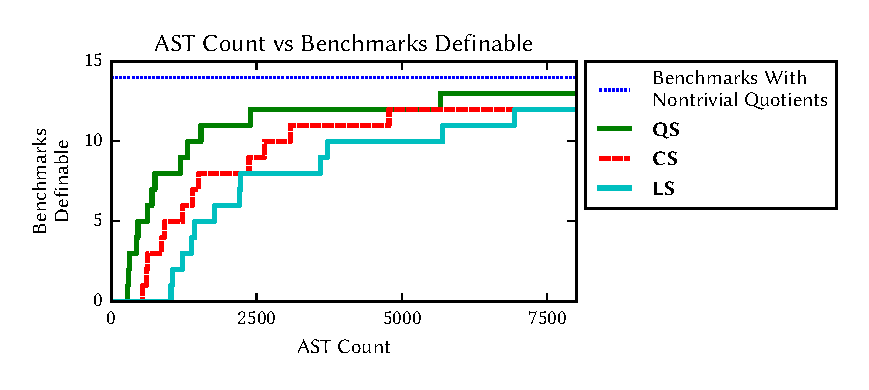
\includegraphics{generated-graphs/asts.eps}
\caption{AST node measurements for each of the three approaches
on each of the 10 non-bijective benchmark problems.
Benchmarks are sorted in order of increasing complexity as measured by
the number of AST nodes in the source and target format descriptions. 
QRE Synthesis requires far fewer AST nodes than the other
two approaches.}
%%\caption{Count of benchmark programs definable using a given AST count. We find
%%that it takes far fewer AST nodes to define benchmark lenses using QRE
%%synthesis than with Optician without QRE synthesis or without synthesis.}
\label{fig:asts}
\end{figure}

To evaluate the impact of QRE lens synthsis on programmer effort,
we focus our attention on the 10 problems in the benchmark suite that
are not bijective and hence require non-trivial canonizers. 
(Optician already handles the other problems with minimal programmer
effort.)

We are interested in comparing three different approaches, which vary
in the amount of synthesis used. 
In the first approach, which we call \QRESize{} for QRE Synthesis, the programmer uses
QRE lens synthesis.  She must write QRE specifications of the source and
target formats and she may give examples.
In the second approach, which we call \canonizeAndSpecSize{} for
Bijective Synthesis, the
programmer uses bijective lens synthesis \`a la Optician.
She must write canonizers by hand, along with 
regular expressions to describe the external
representations of the source and target formats. (The internal
formats can be inferred from the canonizers.) She may also
provide examples to help in the synthesis of the bijective lens.
In the third approach, which we call \LensAndSpecSize{} for No Synthesis, the
programmer writes the lens between the source and target formats
entirely by hand, including the descriptions of the source and target
formats.

For each problem in the benchmark suite, we calculate the following
measures as proxies for the level of programmer effort when using each
the three approaches:

%
\begin{itemize}
  \item[\QRESize{}:] 
  The number of AST nodes in the QRE specifications for the source and
  target formats, including examples. 
  \item[\canonizeAndSpecSize{}:] 
  The sum of (1) the number of AST nodes in $W(q)$ for each QRE $q$ in the source and target
  formats, (2) the number of AST nodes in $\canonize(q)$ for each QRE $q$ with a
  non-trivial canonizer, and (3) the number of AST nodes in the
  examples.  We use (1) to estimate the burden of describing
  the external source and target formats and (2) to estimate the
  burdern of writing the requisite canonizers
  by hand.  We count the nodes in the examples because they would be
  fed to the bijective synthesizer.  
  These counts are an approximation, as both $W(q)$ and $\canonize(q)$ are
  automatically generated from the corresponding QRE $q$, and it is
  possible that a human-written version might be smaller.
  \item[\LensAndSpecSize{}:] The sum of (1) the number of AST nodes in
  $W(q)$ for each QRE $q$ in the source and target formats and (2) the
  number of AST nodes in the synthesized QRE lens.  We use (1) to
  estimate the burdern of describing the source and target formats
  and (2) to estimate the burdern of writing the appropriate lens by
  hand. These counts are also approximations, as
  $W(q)$ and the synthesized lens may be larger than one written by hand.
\end{itemize}

Figure~\ref{fig:asts} shows each of these measures for the 10
non-bijective problems in the benchmark suite.  On
average (using a geometric mean), \canonizeAndSpecSize{} used~38.5\% more AST nodes
than \QRESize{}, requiring an average of~214 more AST nodes. On 
average, \LensAndSpecSize{} used~180\% more AST nodes than \QRESize{}, requiring an
average of~998 more AST nodes. These figures suggest that introducing QREs saves
programmers significant effort compared to both Optician and basic
Boomerang.

\subsection{Maintaining Competitive Performance}

\begin{figure}[t]
\centering
\begin{subfigure}[b]{.49\textwidth}
\centering
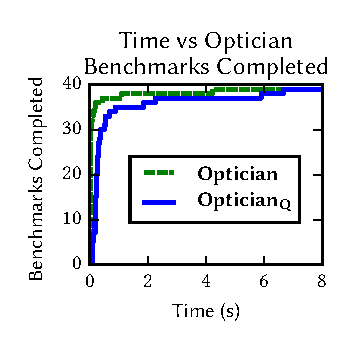
\includegraphics{generated-graphs/times_opt}
\caption{}
\label{subfig:lenssize}
\end{subfigure}
\begin{subfigure}[b]{.49\textwidth}
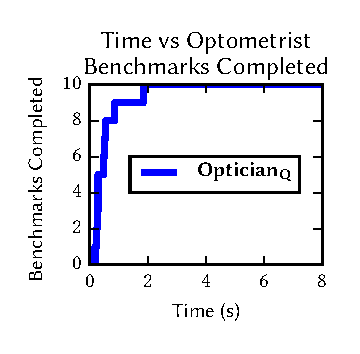
\includegraphics{generated-graphs/times_new.eps}
\caption{}
\label{subfig:examplesused}
\end{subfigure}
\caption{Runtimes measurements. In (a), we run Optician and \QOpt{}
  on the Optician benchmarks.  We find that there is only a negligible
  performance overhead incurred by using QREs. 
  In (b), we run \QOpt{} on the 10 Optician benchmarks
  previously edited to make them bijective, after removing those edits
  and then extending the synthesis specification to include QREs.
  (In other words, we restored them to their original state, added QREs,
  and then ran \QOpt{}). 
  We find that \QOpt{} is able to
  synthesize all quotient lenses in under 10 seconds, and typically finishes in
  under 5 seconds.}
\label{fig:times}
\end{figure}

To assess the performance of QRE synthesis, we are interested in two different
questions. First, how does the performance of \QOpt{} compare to the performance
of Optician on benchmarks that do not require QREs? The answer to this question
tells us how much overhead we have introduced by adopting the more general
mechanism. Figure~\ref{fig:times}(a) shows that \QOpt{} was able to synthesize
all of the Optician benchmarks at a speed competative with the old version.
There is a small amount of additional overhead introduced by QREs in calculating
the $W$ and $K$ functions, resulting in a slight decrease in performance.

Second, how much time does it take for \QOpt{} to synthesize a QRE
lens when running on a non-bijective benchmark problem?  
Figure~\ref{fig:times}(b) shows the amount of time required to infer a
lens for each of the 10 benchmark programs with nontrivial quotients.  
We find that \QOpt{} is able to synthesize all quotient lenses in
under 10~seconds, and typically finishes in under 5~seconds.

\section{Related Work}
\label{relwork}
This paper builds on the work of Foster et al~\cite{quotientlenses} who
introduced the theory of quotient lenses and implemented quotient lenses as a
refinement of the bidirectional string processing language
Boomerang~\cite{boomerang}. As we mentioned in
Section~\ref{subsec:well-formed-qres}, all our QRE combinators can be expressed
using just the {\em normalize} combinator, which is one of the canonizer
primitives that Boomerang already supports. Also, all our QRE lens combinators
are already supported in Boomerang. Consequently Boomerang quotient lenses are
at least as expressive as our language of QRE lenses. 

Boomerang's canonizers allow one to canonize a regular language $R$ to by
mapping it to another regular language $S$ which may not be contained in $S$.
Formally, given sets $C$ and $B$ and an equivalence relation on $B$, Foster et
al defined a {\em canonizer} $q$ from $C$ to $B/{\equiv_B}$ to be a pair of
functions $q.\kw{canonize} : C \longrightarrow B$ and $q.\kw{choose} : B
\longrightarrow C$ such that for every $b \in B$:
$$q.\kw{canonize} \; (q.\kw{choose} \; b) \equiv_B \; b$$
This definition gives allows much more latitude for defining canonizers than
QREs. For example, if $\equiv_B$ is equal to $\kw{Tot}(B)$, the equivalence
relation that relates every element in $B$ to every other element in $B$, then
every function from $C$ to $B$ is a canonizer.

Because of this extra elbow-room, Boomerang is able to offer two primitive
{\em duplication} quotient lenses, the first of which can be derived using
the following inference rule,
\begin{prooftree}
\AxiomC{$\ell : C/{\equiv_C} \Leftrightarrow A_1/{\equiv_{A_1}}$}
\AxiomC{$f : C \longrightarrow A_2$}
\AxiomC{$A_1 \cdot^! A_2$}
\AxiomC{$\equiv_A = \equiv_{A_1} \cdot \kw{Tot}(A_2)$}
\QuaternaryInfC{$\kw{dup}_1 \ell \; f \; : \; C/{\equiv_C} \Longrightarrow A_1
\cdot A_2/{\equiv_A}$}
\end{prooftree}
\begin{align*}
(\kw{dup}_1 \; \ell \; f).\get \; c &= (\ell.\get \; c) \cdot (f \; c)\\
(\kw{dup}_1 \; \ell \; f).\lput \; (a_1 \cdot a_2) \; c &= \ell.\lput \; a_1 \; c\\
(\kw{dup}_1 \; \ell \; f).\create \; (a_1 \cdot a_2) &= \ell.\create \; a_1
\end{align*}
with the symmetric $\kw{dup}_2$ combinator discarding the first copy instead of
the second in the \lput/\create{} direction. 

Boomerang's more general definition for canonizers also allows quotient lenses
to be used as canonizers by using the taking the \kw{canonize} function to be
the \get{} component of a lens and the \kw{choose} function to be its \create{}
component. Naturally, QREs also take advantage of this ability to use lenses as
canonizers by allowing for user-defined functions to be used by the \kw{squash}
and \kw{normalize} combinators. Moreover, the added functionality of
synthesizing lenses further makes it easier to define canonizers, as well as
lenses.

Foster et al also discuss other bidirectional programming languages that
support quotienting of data including XSugar~\cite{xsugar}, biXid~\cite{bixid}
and X/Inv~\cite{Hu2004,Mu2004,Mu2006}; we refer the reader to the related work
section in \cite{quotientlenses} for this discussion.

A newer language which supports quotenting is BiFluX~\cite{pacheco2014biflux}, a
bidirectional functional update language for XML. BiFluX is inspired by
the FLUX XML update language~\cite{cheney2008flux}, and adopts a bidirectional
programming by update paradigm, where a program succintly and precisely
describes {\em how} to update a source document with a target document, in an
intuitive way, such that there is a unique ``inverse'' source query for each
update program. The source and view types of BiFluX programs are given by
regular expressions.

In BiFluX, a regular expression $R$ is said to be unambiguous if there is only
one way to parse a {\em flat} value of type $R$ to a stuctured value of type
$R$; here a flat value of $R$ is a value of $R$ with all left/right tags,
parantheses and list brackets removed. The bidirectional part of BiFluX involves
transforming source regular expressions to view regular expressions so that
data sequences described by the two types can be matched. This process can
result in intermediate types that are ambiguous, and this ambiguity can cause
unintended updates to be made the source, especially when information is
discarded in this process.

\iffalse
For example, imagine that a book database has source type \\
$S$ = \lstinline{books[book[title[string], author[string]+]*]}
with view type $V$ = \lstinline{title[string]}. When the source type is
transformed to the view type for matching, only titles are kept, the element
labels are destroyed and all authors are replaced for the empty sequence, thus
leaving the intermediate type $S'$ = \lstinline{(title[string],(),()*)*}. In
BiFluX, $V$ is considered a subtype of $S'$ because the flat values of $V$ are
also flat values of $S'$. Since the intermediate type is $S'$ ambiguous, a view
sequence \lstinline{[title["mybook"]]} would be upcast into an intermediate
value \lstinline{[(title["mybook"],((), [ ]))]} that would in turn lead to an
updated source \lstinline{books[[book[(title["mybook"],(aut, [ ]))]]]}, which is
clearly unsatisfactory as it would discard the entire book database except the
first author \lstinline{aut} of the first book.
\fi
The typechecking phase of a BiFluX program therefore includes a {\em type
normalization} phase that tries to normalize a source types using automata
reduction techniques, and derive a lens between ambiguous and unambiguous
types. On the view side, this phase only tries to normalize view types into
isomorphic types. Pacheco et. al. do not claim that their normalization
procedures are complete in the sense that they can disambiguate any ambiguous
type, but they do show that when these procedures succed the normalized types
are unambiguous.

{\em Formlenses}~\cite{rajkumar2014lenses} are a variant of lenses that
perform transformations up to equivalence. Formlenses are a bidirectional
generalization of {\em formlets}~\cite{cooper2008essence}, which are a
high-level abstraction for building Web forms. Formlets encapsulate several
low-level details including selecting field names for elements and parsing data
from client responses. In their work, Rajkumar et. al. represent formlets as
functions that take a source of names---concretely, an integer $n$ that should
be used as the next name---as an argument and produce a triple consisting of an
HTML document, a {\em collect} function, and a modified namesource:
\begin{center}
\begin{lstlisting}
type Formlet a = Int $\to$ (Html, Env $\to$ a, Int)
\end{lstlisting}
\end{center}
The names of any generated form fields are drawn from the namesource, and the
{\em collect} function looks up precisely these names. For example the
\kw{inputInt} combinator below builds a form that accepts an integer,
\begin{center}
\begin{lstlisting}
inputInt :: Formlet Int
inputInt i = let n = show i in
             ($\kw{inputTag}$ {name = n, value = ""},$\lambda e \longrightarrow \kw{read}$ ($\kw{fromJust}$ ($\kw{lookup}$ n e)),i+1)
\end{lstlisting}
\end{center}
where \kw{inputTag} constructs an input element, \kw{lookup}
retrieves a value from an association list \kw{fromJust} extracts the
encapsulated value from a \kw{Maybe} value, and \kw{read} parses an \kw{Int}
from a \kw{String}.

Rajkumar et. al. observe that formlets are a useful abstraction, but they only
address one half of the problem---they make it easy to construct a function
that {\em produces} a value of type \codefont{a}, but they do not provide a way
to describe a function that {\em consumes} a value of type \codefont{a} and
embeds it in a form. A different way to think about this problem is to observe
that forms are often used to present an {\em updateable view} of the data
source. Therefore, Rajkumar et. al. leverage the power of bidirectional
transformations to define formlets that behave like updatable views, yielding
the abstraction of formlenses.

The Formlens type is given by
\begin{center}
\begin{lstlisting}
type Formlens a = Maybe a $\to$ [Int] $\to$ (Html,Env $\to$ Maybe a,[Int])
\end{lstlisting}
\end{center}
with the differences between this definition and the standard definition for
formlets being an extra \codefont{Maybe\; a} parameter that provides an
optional initial value of the form, the namesource being changed to a list of
integers, and the {\em collect} function being allowed to return an optional
value.

Rajkumar et. al. consider only formlenses that are well-formed in that a
well-formed formlens should only draw names from the namesource provided as an
argument, and the {\em collect} function should only look up corresponding
names. Under this assumption, Rajkumar et. al. define what it means for a
formlens to be well behaved by defining a version of the classical
\textsc{GetPut} and \textsc{PutGet} laws for formlenses. These laws hold modulo
an equivalence relation on environments, since a formlens may be invoked with
two separate namespaces, but this should not affect the value stored in the
information encapsulated in the type $a$. Consequently, the \textsc{GetPut} and
\textsc{PutGet} laws defined for formlenses are in spirit analogous to the
\textsc{GetPut} and \textsc{PutGet} laws for quotient lenses, since they hold
up to renaming of environment variables.

\iffalse
Well-behaved formlenses satisfy properties that are analogous to the classical
\textsc{GetPut} and \textsc{PutGet} law. If {\em extract} is a function from
\kw{Html} to \kw{Env} that extracts an environment containing the names and
values of all the form fields from an HTML document, then a formlens $f$
satisfies the Acceptability law if for any $v$ of type $a$, $n$ of type
\kw{Int} and environment $e$ of type \kw{Env} if $f$ applied to \kw{Just v} and
$n$ yields an HTML file $h$ and a {\em collect} function $c$ where \kw{extract
h} is contained in $e$, then collect $e$
\fi
Another recent line of work that exploits equivalence relations on data is by
Hilken et. al. in \cite{hilken2016testing}. This work is concerned mainly with
testing, and uses {\em Equivalence Partitioning}, a software testing technique
that divides the input data of a software unit into partitions of equivalent
data from which test cases can be derived. This approach has the advantage that
it can greatly reduce the number of test cases and hence the amount of time
spent testing since only one representative from each class is tested.

More concretely, their approach gives the developer an explicit option to
formulat her understanding of two object models being different. The technical
realization is as follows: The developer specifies ``classifying term'', a
closed Object Constraint Language (OCL) query term that can be evaluated in an
object model and returns a characteristic value. Two object models with the same
characteristic value belong to the same equivalence class. For example under a
configuration requiring at least 2 and at most 4 Person objects, the
classifying term \lstinline{Person.allInstances()->size()} would yield three
object models with 2,3 and 4 Person objects respectively.

Classifying terms are therefore analogous to our QREs or to Boomerang canonizers
in the sense that they define an equivalence relation on data. However, while
QREs and canonizers aim at identifying or characterizing the elements that
should be treated equally by a lens, the focus of the work by Hilken et. al. is
on classes that represent specific patterns of particular relevance to the
modeler who is interested in analyzing the behavior of a transformation.

Finally, Cunha~\cite{cunha2010relational} uses relational algebra to encompass
many of the existing approaches to bidirectional programming. For example,
using $\circ$ to express relational composition, the \textsc{GetPut} law states
that $\get \circ \lput \subseteq \equiv_V \circ \pi_1$, where $\pi_1$ is the
projection onto the first factor. In addition to its generality, this
``point-free'' approach to defining bidirectional transformations has the
advantage of creating equational proofs of lens laws that proceed by folding
and unfolding combinator laws.

Next we turn to related work in program synthesis. Much of the research in
synthesis assumes that the synthesizer is provided with a collection of examples.
Optician and Optician$_Q$ differ in that they require the programmer to supply
both examples {\em and} format descriptions in the form of regular expressions
or QREs, though these two systems are far from the only ones to consider
type-based synthesis. There is a trade-off here.  On the one hand, a user must
have some programming expertise to write regular expression (or QRE)
specifications, and it requires some work. On the other hand, such
specifications provide a great deal of information to the synthesis system,
which decreases the number of examples needed (often to zero), makes the system
scale well, and allows it to handle large, complex formats.  By providing these
format specifications, the synthesis engine does not have to both infer the
format of the data as well as the transformations on it, obviating the need to
infer tricky formats like those involving nested iterations. 

There are many other recent results showing how to synthesize functions from
type-based
specifications~\cite{augustsson-2004,osera+:pldi15,feser-pldi-2015,scherer-icfp-2015,frankle+:popl16,armando+:pldi16}.
These systems enumerate programs of their target language, orienting their
search procedures to process only terms that are well-typed.
Optician is distinctive in that it synthesizes terms in a language with many
type equivalences. Perhaps the system most similar to Optician is
InSynth~\cite{gvero-pldi-2013}, a system for synthesizing terms in the
simply-typed lambda calculus that addresses equivalences on types. Instead of
trying to directly synthesize terms of the simply-typed lambda calculus,
InSynth synthesizes a well-typed term in the succinct calculus, a language with
types that are equivalent ``modulo isomorphisms of products and
currying''~\cite{gvero-pldi-2013}. The type structure used in Optician
is significantly more complex.  In particular, because Optician types do not
have full canonical forms, Anders et. al. used a pseudo-canonical form that
captures part of the equivalence relation over types were used. To preserve
completeness, they pushed some of the remaining parts of the type equivalence
relation into a set of rewriting rules and other parts into the synthesis
algorithm itself.

Morpheus~\cite{morpheus} is another synthesis system that uses two
communicating synthesizers to generate programs.  In both Morpheus and
Optician, one synthesizer provides an outline for the program, and the other
fills in that outline with program details that satisfy the user's
specifications. This approach works well in large search spaces that require
some enumerative search. One important way that Optician differs from Morpheus
is that in Morpheus, an outline is a sketch---an \emph{expression}
containing holes---whereas an outline in Optician is a pair of regular
expressions, i.e., a \emph{type}.  Moreover, in order to implement an efficient
search procedure, Anders et. al had to create both a new type language and a new
term language for lenses.  Once they did so, they proved their new, more
constrained language designed for synthesis was just as expressive as the
original, more flexible and compositional language designed for human
programmers.

\section{Conclusion and Future Work}
\label{concl}

In this paper, we showed how to synthesize a class of bijective quotient lenses
using the bijective lens synthesis system Optician as a plug-in for our
synthesis algorithm. In order to achieve this, we first introduced {\em
Quotient regular languages} to specify regular languages with an equivalence
relation defined on them. Then, we introduced {\em QRE lenses}, which
are bijective quotient lenses that map between QREs via bijective lenses. We
proved a normal form theorem for QREs that enabled us to (1) extend the
synthesis algorithm used by Optician to synthesize QRE lenses, and (2) prove
that if there is a QRE lens that satisfies the input specification, then the
extended algorithm returns such a lens. Finally we tested QRE-enhanced optician
on the Optician benchmark suite and demonstrated that QREs can save programmers
significant effort compared to both Optician and basic Boomerang, and that
QRE-enhanced Optician maintains competitive performance over both of these
systems.

Looking ahead, we are experimenting with larger examples of
quotiented bijective lenses.  So far, the three ``specialized'' QRE
combinators (\kw{squash}, \kw{perm}, and \kw{collapse}) have proved
sufficient, but we expect eventually to encounter examples that will lead us
to consider adding further combinators to supplement these.

Along a different dimension, we would like to investigate whether the techniques
proposed here can be applied to synthesizing quotiented variants of richer
classes of lenses, such as ``classic'' asymmetric lenses~\cite{Lenses} or
symmetric lenses~\cite{hofmann2011symmetric}.  The main technical issues are
developing synthesis procedures for the unquotientied variants of a given
class---we are currently attacking the case of symmetric lenses---and showing
that quotiented lenses in this class can be normalized along the lines of
Theorem~\ref{normal form}.

\bibliographystyle{plain}
\bibliography{local}

\appendix
\addcontentsline{toc}{section}{Appendices}
\section*{Appendices}
\section{Proof of Normal Form Theorem for QRE lenses}
\cref{normal form} claims that if there is a derivation $q : Q_1
\Leftrightarrow Q_2$, then there exists a bijective lens $\ell : K(Q_1)
\Leftrightarrow K(Q_2)$ such that:
\begin{align*}
\llbracket q \rrbracket.\get &= \llbracket \ell \rrbracket\circ
\canonize(Q_1)\\
\llbracket q \rrbracket.\lput &= \llbracket \ell \rrbracket^{-1} \circ
\canonize(Q_2)
\end{align*}
We now prove this theorem.
\begin{proof}
We proceed by induction over the derivation $q : Q_1 \Leftrightarrow Q_2$.
\begin{enumerate}
  \item
  $\kw{lift}(\ell): R/\mathit{id}(R) \Leftrightarrow S/\mathit{id}(S)$ where
  $\ell : R \Leftrightarrow S$. Then:
  \begin{align*}
\llbracket \kw{lift}(\ell) \rrbracket.\get &=  \llbracket \ell \rrbracket
= \llbracket \ell \rrbracket \circ id_{\mathcal{L}(R)} =
\llbracket \ell \rrbracket \circ \canonize(\mathit{id}(R)), \text{ and }\\
\llbracket \kw{lift}(\ell) \rrbracket.\lput &= \llbracket \ell
\rrbracket^{-1} = \llbracket \ell \rrbracket^{-1} \circ id_{\mathcal{L}(S)} =
\llbracket \ell \rrbracket^{-1} \circ \canonize(id(S))
\end{align*}
\item
$\lquot(Q_1, q): Q_1 \; ; \; Q_2 \Leftrightarrow Q_3$ where $q : Q_2
\Leftrightarrow Q_3$, $Q_1$ is well formed and $K(Q_1) = W(Q_2)$. Then:
\begin{align*}
\llbracket \lquot(Q_1, q) \rrbracket.\get  &= \llbracket q
\rrbracket.\get \circ \canonize(Q_1)\\
\llbracket \lquot(Q_1, q) \rrbracket.\lput &= \llbracket q \rrbracket.\lput
\end{align*}
By the induction hypothesis, there exists a bijective lens $\ell :
K(Q_2) \Leftrightarrow K(Q_3)$ such that:
\begin{align*}
\llbracket q \rrbracket.\get &= \llbracket \ell \rrbracket \circ
\canonize(Q_2)\\
\llbracket q \rrbracket.\lput &= \llbracket \ell \rrbracket^{-1} \circ
\canonize(Q_3)
\end{align*}
Consequently
\begin{align*}
\llbracket \lquot(Q_1, q)\rrbracket.\get  &= (\llbracket \ell \rrbracket \circ
\canonize(Q_2)) \circ \canonize(Q_1) = \llbracket \ell \rrbracket \circ
(\canonize(Q_1 \; ; \; Q_2))\\
\llbracket \lquot(Q_1, q) \rrbracket.\lput &= \llbracket \ell \rrbracket^{-1}
\circ \canonize(Q_3)
\end{align*}

\item
$\rquot(q, Q_3):Q_1 \Leftrightarrow Q_2 \; ; \; Q_3$ where $q : Q_1
\Leftrightarrow Q_2$, $Q_3$ is well formed and $K(Q_3) = W(Q_2)$. Proceed as in
the previous case.
\item
$q_1 \; ; \; q_2: c \Leftrightarrow Q_2$ where $q_1 : c \Leftrightarrow Q_1$ and
$q_2 : Q_1 \Leftrightarrow Q_2$. Then:
\begin{align*}
\llbracket q_1 \; ; \; q_2 \rrbracket.\get &= \llbracket q_2
\rrbracket.\get\circ \llbracket q_1 \rrbracket.\get, \text{ and }\\
\llbracket q_1 \; ; \; q_2 \rrbracket.\lput &= \llbracket q_1 \rrbracket.\lput
\circ \llbracket q_2 \rrbracket.\lput
\end{align*}
By the induction hypothesis, there exist bijective lenses,
$\ell_1 :
K(c) \Leftrightarrow K(Q_1)$ and $\ell_2 : K(Q_1) \Leftrightarrow K(Q_2)$ such
that,
\begin{align*}
\llbracket q_1 \rrbracket.\get &= \llbracket \ell_1 \rrbracket \circ
\canonize(c)\\
\llbracket q_1 \rrbracket.\lput &= {\llbracket \ell_1 \rrbracket}^{-1} \circ
\canonize(Q_1)
\end{align*}
and
\begin{align*}
\llbracket q_2 \rrbracket.\get &= \llbracket \ell_2 \rrbracket \circ
\canonize(Q_1)\\
\llbracket q_2 \rrbracket.\lput &= {\llbracket \ell_2 \rrbracket}^{-1} \circ
\canonize(Q_2)
\end{align*}
Consequently:
\begin{align*}
\llbracket q_1 \; ; \; q_2 \rrbracket.\get &=
\llbracket q_2 \rrbracket.\get \circ \llbracket q_1 \rrbracket.\get \\
&=(\llbracket \ell_2 \rrbracket \circ \canonize(Q_1)) \circ (\llbracket \ell_1
\rrbracket \circ \canonize(c))\\
&= \llbracket \ell_2 \rrbracket \circ (\canonize(Q_1) \circ \llbracket \ell_1
\rrbracket) \circ \canonize(c)\\
&= (\llbracket \ell_2 \rrbracket \circ \llbracket \ell_1 \rrbracket) \circ
\canonize(c)\\
&= \llbracket \ell_1 \; ; \; \ell_2 \rrbracket \circ
\canonize(c)
\end{align*}
A similar argument shows that:
$$\llbracket q_1 \; ; \; q_2 \rrbracket.\lput =
\llbracket \ell_1 \; ; \; \ell_2 \rrbracket^{-1} \circ
\canonize(c)$$
\item
$q^* : {Q_1}^* \Leftrightarrow {Q_2}^*$ where $q : Q_1 \Leftrightarrow Q_2$,
$W(Q_1)^{*!}$ and $W(Q_2)^{*!}$ and $K(Q_1)^{*!}$ and $K(Q_2)^{*!}$. Then:
\begin{align*}
\llbracket q^* \rrbracket.\get &= (\llbracket q \rrbracket.\get)^*, \text{
and }\\
\llbracket q^* \rrbracket.\lput &= (\llbracket q \rrbracket.\lput)^*
\end{align*}
By the induction hypothesis there exists a bijective lens $\ell : K(Q_1)
\Leftrightarrow K(Q_2)$ such that:
\begin{align*}
\llbracket q \rrbracket.\get &= \llbracket \ell \rrbracket \circ
\canonize(Q_1)\\
\llbracket q \rrbracket.\lput &= {\llbracket \ell \rrbracket}^{-1} \circ
\canonize(Q_2)
\end{align*}
Consequentlty:
\begin{align*}
\llbracket q^* \rrbracket.\get &= (\llbracket \ell \rrbracket \circ
\canonize(Q_1))^* = \llbracket \ell \rrbracket^* \circ
\canonize(Q_1)^* = \llbracket \ell^* \rrbracket \circ
\canonize(Q_1^*)\\
\llbracket q^* \rrbracket.\lput &= (\llbracket \ell \rrbracket^{-1} \circ
\canonize(Q_2))^* = (\llbracket \ell \rrbracket^{-1})^* \circ
\canonize(Q_2)^* = \llbracket \ell^* \rrbracket^{-1} \circ
\canonize(Q_2^*)\\
\end{align*}
\item
$q_1 \cdot q_2: Q_1 \cdot Q_2 \Leftrightarrow Q_3 \cdot Q_4$, where $q_1 : Q_1
\Leftrightarrow Q_3 $,  $q_2 : Q_2 \Leftrightarrow Q_4$, $W(Q_1)
\cdot^! W(Q_2)$, $K(Q_1) \cdot^! K(Q_2)$, $W(Q_3) \cdot^! W(Q_4)$ and $
K(Q_3) \cdot^! K(Q_4)$. Then:
\begin{align*}
\llbracket q_1 \cdot q_2 \rrbracket.\get &= \llbracket q_1 \rrbracket.\get \cdot
\llbracket q_2 \rrbracket.\get, \text{ and }\\
\llbracket q_1 \cdot q_2 \rrbracket.\lput &= \llbracket q_1 \rrbracket.\lput
\cdot \llbracket q_2 \rrbracket.\lput
\end{align*}
By the induction hypothesis, there exist bijective lenses $\ell_1 : K(Q_1)
\Leftrightarrow K(Q_3)$ and $\ell_2 : K(Q_2) \Leftrightarrow K(Q_4)$ such that,
\begin{align*}
\llbracket q \rrbracket.\get &= \llbracket \ell_1 \rrbracket \circ
\canonize(Q_1)\\
\llbracket q \rrbracket.\lput &= {\llbracket \ell_1 \rrbracket}^{-1} \circ
\canonize(Q_3)
\end{align*}
and
\begin{align*}
\llbracket q_2 \rrbracket.\get &= \llbracket \ell_2 \rrbracket \circ
\canonize(Q_2)\\
\llbracket q_2 \rrbracket.\lput &= {\llbracket \ell_2 \rrbracket}^{-1} \circ
\canonize(Q_4)
\end{align*}
Consequently:
\begin{align*}
\llbracket q_1 \cdot q_2 \rrbracket.\get &= (\llbracket \ell_1 \rrbracket \circ
\canonize(Q_1)) \cdot  (\llbracket \ell_2 \rrbracket \circ
\canonize(Q_2))\\
&= (\llbracket \ell_1 \rrbracket \cdot \llbracket \ell_2
\rrbracket) \circ (\canonize(Q_1) \cdot \canonize(Q_2))\\
&= \llbracket \ell_1 \cdot  \ell_2 \rrbracket \circ \canonize(Q_1 \cdot Q_2)
\end{align*}
Similarly:
$$
\llbracket q_1 \cdot q_2\rrbracket.\lput = \llbracket \ell_1 \cdot  \ell_2
\rrbracket^{-1} \circ \canonize(Q_3 \cdot Q_4) $$
\item
$\swap(q_1,q_2): Q_1 \cdot Q_2 \Leftrightarrow Q_4 \cdot Q_3$, where $q_1 : Q_1
\Leftrightarrow Q_3 $,  $q_2 : Q_2 \Leftrightarrow Q_4$, $W(Q_1)
\cdot^! W(Q_2)$, $K(Q_1) \cdot^! K(Q_2)$, $W(Q_4) \cdot^! W(Q_3)$ and $
K(Q_4) \cdot^! K(Q_3)$. Then:
\begin{align*}
\llbracket \swap(q_1, q_2) \rrbracket.\get(s_1 \cdot s_2) &= \llbracket q_2
\rrbracket.\get(s_2) \cdot \llbracket q_1 \rrbracket.\get(s_1), \text{ and }\\
\llbracket \swap(q_1, q_2) \rrbracket.\lput(t_1, t_2) &= \llbracket q_1
\rrbracket.\lput(t_1) \cdot \llbracket q_2 \rrbracket.\lput(t_2)
\end{align*}
By the induction hypothesis, there exist bijective lenses $\ell_1 : K(Q_1)
\Leftrightarrow K(Q_3)$ and $\ell_2 : K(Q_2) \Leftrightarrow K(Q_4)$ such that,
\begin{align*}
\llbracket q_1 \rrbracket.\get &= \llbracket \ell_1 \rrbracket \circ
\canonize(Q_1)\\
\llbracket q_1 \rrbracket.\lput &= {\llbracket \ell_1 \rrbracket}^{-1} \circ
\canonize(Q_3)
\end{align*}
and
\begin{align*}
\llbracket q_2 \rrbracket.\get &= \llbracket \ell_2 \rrbracket \circ
\canonize(Q_2)\\
\llbracket q_2 \rrbracket.\lput &= {\llbracket \ell_2 \rrbracket}^{-1} \circ
\canonize(Q_4)
\end{align*}
Consequently:
\begin{align*}
\llbracket \swap(q_1, q_2) \rrbracket.\get(s_1 \cdot s_2) &= \llbracket q_2
\rrbracket.\get(s_2) \cdot \llbracket q_1 \rrbracket.\get(s_1)\\
&= (\llbracket \ell_2 \rrbracket \circ
\canonize(Q_2))(s_2) \cdot  (\llbracket \ell_1 \rrbracket \circ
\canonize(Q_1))(s_1)\\
&= (\llbracket \swap(\ell_1, \ell_2) \rrbracket) \circ (\canonize(Q_1) \cdot
\canonize(Q_2)) (s_1, s_2)
\end{align*}
Similarly:
$$
\llbracket \swap(q_1, q_2) \rrbracket.\lput = (\llbracket \swap(\ell_1, \ell_2)
\rrbracket)^{-1} \circ (\canonize(Q_4) \cdot \canonize(Q_3))$$
\item
$q_1 = q_1 \sep q_2$ where $q_1 : Q_1 \Leftrightarrow Q_3 $, $q_2 : Q_2
\Leftrightarrow Q_4$, $\mathcal{L}(W(Q_1)) \cap \mathcal{L}(W(Q_2)) =
\varnothing$ and $\mathcal{L}(W(Q_3)) \cap \mathcal{L}(W(Q_4)) = \varnothing$.
Then:$$
\llbracket q_1 \sep q_2 \rrbracket.\get(s) =
\begin{cases}
\llbracket q_1 \rrbracket.\get (s) & \text{if } s \in \mathcal{L}(W(Q_1))\\
\llbracket q_2 \rrbracket.\get (s) & \text{if } s \in \mathcal{L}(W(Q_2))\\
\end{cases}$$
$$\llbracket q_1 \sep q_2 \rrbracket.\lput(s) =
\begin{cases}
\llbracket q_1 \rrbracket.\lput (s) & \text{if } s \in \mathcal{L}(W(Q_3))\\
\llbracket q_2 \rrbracket.\lput (s) & \text{if } s \in \mathcal{L}(W(Q_4))\\
\end{cases}
$$
By the induction hypothesis, there exist bijective lenses $\ell_1 : K(Q_1)
\Leftrightarrow K(Q_3)$ and $\ell_2 : K(Q_2) \Leftrightarrow K(Q_4)$ such that,
\begin{align*}
\llbracket q_1 \rrbracket.\get &= \llbracket \ell_1 \rrbracket \circ
\canonize(Q_1)\\
\llbracket q_1 \rrbracket.\lput &= {\llbracket \ell_1 \rrbracket}^{-1} \circ
\canonize(Q_3)
\end{align*}
and
\begin{align*}
\llbracket q_2 \rrbracket.\get &= \llbracket \ell_2 \rrbracket \circ
\canonize(Q_2)\\
\llbracket q_2 \rrbracket.\lput &= {\llbracket \ell_2 \rrbracket}^{-1} \circ
\canonize(Q_4)
\end{align*}
Consequently:
$$
\llbracket q_1 \sep q_2 \rrbracket.\get(s) =
\begin{cases}
\llbracket \ell_1 \rrbracket \circ
\canonize(Q_1) (s) & \text{if } s \in \mathcal{L}(W(Q_1))\\
\llbracket \ell_2 \rrbracket \circ
\canonize(Q_2) (s) & \text{if } s \in \mathcal{L}(W(Q_2)),\\
\end{cases}$$
so $\llbracket q_1 \sep q_2 \rrbracket.\get = \llbracket \ell_1 \sep
\ell_2 \rrbracket \circ \canonize(Q_1 \sep Q_2)$. A similar argument shows
that $\llbracket q_1 \sep q_2 \rrbracket.\lput = \llbracket \ell_1 \sep
\ell_2 \rrbracket^{-1} \circ \canonize(Q_3 \sep Q_4)$.\\
This completes the proof. 
\end{enumerate}
\end{proof}

\section{Proof of Correctness of \textproc{SynthQRELens}}
Theorem~\ref{thm:alg-correct} states that
  Given QREs $Q_1$ and $Q_2$, and a set of examples
  $\{(x_1,y_1),\ldots,(x_n,y_n)\}$, if there is a QRE lens $q : Q_1
  \Leftrightarrow Q_2$ such that $q.\get(x_i) \equiv_{Q_2} y_i \text{ and }
q.\lput(y_i) \equiv_{Q_1} x_i$, then $\textproc{SynthQRELens}(Q_1,Q_2,exs)$ will
return such a lens.  We prove that here.

\begin{lemma}[Algorithm Soundness]
  If $q = \textproc{SynthQRELens}(Q_1,Q_2,exs)$, then $q : Q_1 \Leftrightarrow
  Q_2$ and $q.\get(x_i) \equiv_{Q_2} y_i$  and 
$q.\lput(y_i) \equiv_{Q_1} x_i$ for all $(x_i,y_i)\in exs$.
\end{lemma}
\begin{proof}
  As $q = \textproc{SynthQRELens}(Q_1,Q_2,exs)$, we know that $q =
  \rquot(\lquot(Q_1, \ell), Q_2)$. Furthermore, we know that $\ell =
  \Call{SynthBijectiveLens}{R_1,R_2,exs'}$, where $exs' = \Call{Map}{exs,fun \,
    (ex_l,ex_r) \to (\canonize(Q_1)(ex_l),\canonize(Q_2)(ex_r))}$. By the
    correctness of $\textproc{SynthBijectiveLens}$, we know that
    $\ell.\get(x_i') = y_i'$ and $\ell.\lput(y_i') = x_i'$ for all
    $(x_i',y_i')\in exs'$. By definitions of $\rquot$ and $\lquot$, this means
    that:\\
$\rquot(\lquot(Q_1, \ell),
  Q_2).\get(x_i)$\\
 = $\ell.get(\canonize(Q_1)(x_i))$\\ $= \ell.get(x_i') = y_i' =
  \canonize(Q_2)(y_i) \equiv_{Q_2} y_i$ and\\
\\
$\rquot(\lquot(Q_1, \ell),
  Q_2).\lput(y_i)$\\
 = $\ell.\lput(\canonize(Q_2)(y_i))$\\ $= \ell.\lput(y_i') = x_i' =
  \canonize(Q_1)(x_i) \equiv_{Q_1} x_i$ as desired.
\end{proof}

\begin{lemma}[Algorithm Completeness]
  If there exists a QRE lens $q : Q_1 \Leftrightarrow Q_2$ such that
  $q.\get(x_i) \equiv_{Q_2} y_i$ and $q.\lput(y_i) \equiv_{Q_1} x_i$ for all
  $(x_i,y_i)\in exs$, then $\textproc{SynthQRELens}(Q_1,Q_2,exs)$ terminates.
\end{lemma}
\begin{proof}
  By Theorem~\ref{normal form}, there exists a bijective lens $\ell : K(Q_1)
  \Leftrightarrow K(Q_2)$, such that $q' = \rquot(\lquot(Q_1, \ell), Q_2)$ is
  semantically equal to $q$.

  This means that $q'.\get(x_i) \equiv_{Q_2} y_i$ and $q'.\lput(y_i)
  \equiv_{Q_1} x_i$ for all $(x_i,y_i)\in exs$. Unfolding the definitions of
  $\rquot$ and $\lquot$, we get:\\
  $q'.\get(x_i) = \ell.\get(\canonize(Q_1)(x_i)) = \canonize(Q_2)(y_i)$ and\\
  $q'.\lput(y_i) = \ell.\lput(\canonize(Q_2)(y_i)) = \canonize(Q_1)(x_i)$ for all
  $(x_i,y_i)\in exs$.

  By correctness of $\textproc{SynthBijectiveLens}$, we know that
  $\Call{SynthBijectiveLens}{R_1,R_2,exs'}$ terminates, so the entire algorithm
  terminates. 
\end{proof}

With soundness and completeness, we trivially get the correctness theorem.

\end{document}
